%%%%
%% Copyright 2022 Pierre S. Caboche
%% All rights reserved
%%%%

\documentclass[twoside]{article}


%% Packages and their configuration
% Copyright 2022 Pierre S. Caboche. All rights reserved.

%% Packages and configuration

\usepackage{geometry}
\geometry{
	a4paper,
	total={170mm,257mm},
	left=35mm,
	right=35mm,
	top=30mm,
	bottom=30mm,
}


\usepackage{fontspec}
\setmainfont{DejaVu Serif} 
\setsansfont{DejaVu Sans} 

%% Use Sans-Serif by default
\renewcommand{\familydefault}{\sfdefault}


\usepackage{xeCJK}
\setCJKmainfont{Noto Serif JP}
\setCJKsansfont{Noto Sans JP}
\setCJKmonofont{Noto Sans Mono CJK JP}

\usepackage{xpinyin}


%% bibliography
\usepackage[authoryear]{natbib}

%% index
\usepackage{imakeidx}
\makeindex


\usepackage{xcolor}
\usepackage{graphicx}


\usepackage{titleps}
\usepackage{xstring}
\newcommand{\currentPart}{}

\newcommand{\formatPartTitleDefault}{
	\textbf{\IfStrEq{\thepart}{}{}{Part \thepart\ ---  }\currentPart}
}

\newcommand{\formatPartTitle}{\formatPartTitleDefault}

\newcommand{\copyrightNotice}{\color{gray}{\emph{\textcopyright\ 2022 Pierre S. Caboche. All rights reserved.}}}

\newpagestyle{main}{
	\sethead
	% even
	[\formatPartTitle]
	[]
	[]
	% odd
	{}
	{}
	{\formatPartTitle}
	
	\setfoot
	% even
	[\textbf{\thepage\ \color{lightgray}{|}}]
	[]
	[\copyrightNotice]
	% odd
	{\copyrightNotice}
	{}
	{\textbf{\color{lightgray}{|} \color{black}{\thepage} }} 
	
	\headrule
	%\footrule
}
\pagestyle{main}

\widenhead[25pt][25pt]{25pt}{25pt}



\usepackage{listings}
\lstset{
	basicstyle=\fontsize{9}{9}\selectfont\ttfamily
	,frame=lines
	,tabsize=2
	,keywordstyle=\bfseries%\itshape,
	,commentstyle=\itshape\color{teal}
	,stringstyle=\color{magenta}
	,breaklines=true,
	,postbreak=\mbox{\textcolor{red}{$\hookrightarrow$}\space}
}



\usepackage{hyperref}
\usepackage{longtable}
\usepackage[super]{nth}



\widowpenalties 1 10000
\raggedbottom

\setlength{\parindent}{0pt}



%% Custom macros
% Copyright 2022 Pierre S. Caboche. All rights reserved.

\usepackage{mdframed}
\mdfsetup{
	%innertopmargin=10pt,
	frametitleaboveskip=-\ht\strutbox,
	frametitlealignment=\center
}


\newcommand{\note}[1]{
	\mdfsetup{
		middlelinewidth=2pt,
		backgroundcolor=yellow!10
	}
	\begin{mdframed}#1\end{mdframed}
	\mdfsetup{
		backgroundcolor=white
	}
}


\newcommand{\cmd}[1]{\lstinline|#1|}


\newcommand{\python}{Python}
\newcommand{\awk}{AWK}
\newcommand{\perl}{Perl}
\newcommand{\julia}{Julia}
\newcommand{\gawk}{\texttt{gawk}}
\newcommand{\mawk}{\texttt{mawk}}
\newcommand{\sed}{\texttt{sed}}
\newcommand{\grep}{\texttt{grep}}

\newcommand{\stdin}{\texttt{stdin}}
\newcommand{\stdout}{\texttt{stdout}}
\newcommand{\stderr}{\texttt{stderr}}

\newcommand{\mysqldump}{\texttt{mysqldump}}
\newcommand{\cat}{\texttt{cat}}
\newcommand{\pv}{\texttt{pv}}
\newcommand{\shell}{\texttt{shell}}

\newcommand{\Unix}{UNIX\textregistered}
\newcommand{\Intel}{Intel\textregistered}
\newcommand{\Core}{Core\texttrademark}




%opening

\begin{document}

\maketitle





\begin{abstract}
This article condenses all the things I've learned about \LaTeX\ while being stuck at home during the coronavirus pandemic. This guide will help you get started with \LaTeX, so you can focus on the content of your document / thesis / book, etc. \\


This document is self-describing: if you see something in this paper and wonder \emph{``how do we do that in \LaTeX?"} then the answer is likely to be explained somewhere in there. \\


I am no \LaTeX\ expert by any stretch of the imagination; but what I know, I've put in this document. I've also tried to structure the document in a way that is easy to follow (step by step, from an empty template, important features first), even with no prior experience of \LaTeX. \\
 
Enjoy!
\end{abstract}


\newpage
%%%%
%% Copyright 2022 Pierre S. Caboche
%% All rights reserved
%%%%

\part{Preamble}

\section{Introduction}

Every article tells a story, and this one is no different. \\

In this story, we go from being a complete \LaTeX\ novice, to writing documents like this one. 
Starting from nothing, we learn how to install a \LaTeX\ environment (for Windows or Linux), install \TeXstudio, create a new document, render it, then add all the necessary components to make a good report: sections, Table of Contents, cross-references, bibliography, index\dots \\

So this is the story about a \LaTeX\ document, talking about itself: many of the techniques used to produce this document are featured in this document, including some code samples. \\

In any case, sit back, relax, and enjoy the ride through our discovery of \LaTeX\dots 





\newpage
\section{Legal}
\input{"READ_ME_(LEGAL).txt"}


\newpage
%% Customise the title of the Table of Contents (default: Contents)
\renewcommand*\contentsname{Table of Contents}

%% Limit the depth of the TOC
\addtocontents{toc}{\setcounter{tocdepth}{3}}
\setcounter{tocdepth}{3}

%% Print the Table of Contents
\tableofcontents



\newpage
%%%%
%% Copyright 2022 Pierre S. Caboche
%% All rights reserved
%%%%

\part{\LaTeX}

In this part, we will explain what \LaTeX\ is, when to use \LaTeX\ (and why), and compare it with other software.

\section{What is \LaTeX?}

\LaTeX\ is a software system for document preparation. \\
Instead of using formatted text like in a \WYSIWYG\ ("What You See Is What You Get") word processors (such as LibreOffice Writer), the user writes \LaTeX\ code (in plain text) which then can be processed to generate a document. \\

This approach has many advantages. For example, \LaTeX\ allows to define programmable macros to help with recurring tasks (formatting and others); \LaTeX\ provides thousands of packages that cover a variety of domains; and because \LaTeX\ code is written in plain text, it can be managed just like any other source code (so you can use tools like GIT or SVN for collaboration and version control). \\

For all these reasons, \LaTeX\ is widely used in academia, and in many fields like: mathematics, computer science, engineering, physics, chemistry, etc. \LaTeX\ is also used for the preparation and publication of books. \\

Compared to \WYSIWYG\ word processors, \LaTeX\ may have a steeper learning curve but it can also do much more, and can greatly improve productivity in certain cases (e.g. technical articles, which require consistency in styling, the handling of multiple references, etc.). \\
This article will help you get started with \LaTeX, covering a number of subjects needed to write a paper like this. \\

As a rule, this document is self-describing, i.e.: this document was written in \LaTeX, and every technique used to produce this document is explained somewhere in this document.


\subsection{Differences between \TeX, \LaTeX, and others}

The original \TeX\ was created in the late 1970s by Donald Knuth, who needed a new typesetting program. 

\emph{At that time, Knuth was revising the second volume of his book \emph{``The Art of Computer Programming"},  got the galleys from his publisher, and was very disappointed in the result. The quality was so far below that of the first edition that he couldn't stand it. Around the same time, he saw a new book that had been produced digitally, and thought he could produce a digital typesetting system. So he started to learn about typography, type design, and the rules for typesetting math} \citep{tug}\footnote{I highly recommend you look at \cite{tug} if you want to learn more about the history of \TeX}, and thus started his work on \TeX.

\begin{note}
The idea behind \TeX\ was \emph{``to allow anybody to produce high-quality books with minimal effort, and to provide a system that would give exactly the same results on all computers, at any point in time"} \citep{wiki-tex}
\end{note}



The commands in \TeX\ were basic, but allowed the creation of macros to extend the list of commands. \\

In the early 1980s, Leslie Lamport created \LaTeX, a typesetting program written in the \TeX\ macro language. \citep{wiki-latex} 
As such, \LaTeX\ provides a large set of macros for \TeX\ to interpret, and \TeX\ is in charge of formatting the output.


\LaTeX\ packages are centralised in a repository called ``The Comprehensive \TeX\ Archive Network" (CTAN), \emph{``the central place for all kinds of material around \TeX"} %\citep{CTAN}.
%
\begin{note}
	
Broadly speaking, you can think of \LaTeX\ as: \emph{``\TeX, enhanced with a huge collection of macros: more than 6000 packages to date in \cite{CTAN}."}
\end{note}


In 1989, Knuth declared that \TeX\ was feature-complete, and only bug fixes would be made \citep{tex-vs-latex}. Since then, new typesetting programs based on \TeX\ appeared: \pdfTeX, \XeTeX, \LuaTeX\dots\\

When those typesetting programs are used in conjunction with the \LaTeX\ macros, we talk of:  \pdfLaTeX, \XeLaTeX, \LuaLaTeX\dots \\

The advantage of \XeTeX\ (and therefore \XeLaTeX) is that:
\begin{itemize}
	\item \XeTeX\ supports UTF-8 by default
	\item \XeTeX\ can make use of the fonts that are installed on your computer (not just the standard \LaTeX\ fonts)
\end{itemize}

We'll be using \XeLaTeX, so we can use the fonts that are installed on our system. \\




\section{Why use \LaTeX?}

In this part, we show some examples where \LaTeX\ is really beneficial. Conversely, we also discuss cases where better alternatives exist.

Then we discuss how some recent technological improvements made the \LaTeX\ experience a lot more enjoyable than it was about a decade ago. \\

All of this should help you understand \LaTeX\ better, so you can make an informed decision.


\subsection{When is \LaTeX\ a good choice?}

\LaTeX\ is a good choice in the following cases\dots

\begin{description}
	\item[When you have large documents] \mbox{} \\
	If your document contains a lot of parts or chapters, you can break them down in files which are easier to manage, organise (i.e. changing the order of such chapters), and collaborate on (section \ref{getting-organised}).

	\item[When you need to manage cross-references, bibliography, indexes\dots] \mbox{} \\
	We'll explain how these work in sections ``\longref{cross-references}", ``\longref{add-biblio}", and ``\longref{add-index}".
	
	\item[When the style needs to be consistent throughout] \mbox{} \\
	If some elements need to always be formatted in a certain way, write a macro for that. If later you need to change the style, modify the macro and the change will be reflected throughout the whole document.
	
	\item[When you find recurring patterns in your document] \mbox{} \\
	Macros are great to avoid having to perform the same task multiple times: define a macro once, then call it whenever necessary (sometimes with different parameters). 
	
	In part ``\longref{macros}" we explain how macros work, and give a few usage examples.
	
	
	\item[When you have a lot of mathematical formulas] \mbox{} \\
	\LaTeX\ is really good for adding (and referencing) mathematical formulas! However, I will not cover this subject (I did not use any formulas in this article).
		
	\item[When you need to show a lot of source code] \mbox{} \\
	One thing I \emph{did} use, however, is the ability to easily add code samples to a document (with some syntax highlighting for a variety of computer languages), whether it be small snippets of code, or entire source file.
	
	More details in part ``\longref{showing-code}".
	
	
	\item[When you find a \LaTeX\ package that does exactly what you need] \mbox{} \\
	This is a generalisation of the previous point, which uses a specialised package to print some source code from a variety of languages.
	
	With thousands of different packages, it is possible you may find one that suits your need exactly, and that package may save you a lot of time down the line. When that happens, the time spent learning how to use \LaTeX\ is only a small investment, which will be entirely recouped almost immediately.
	
	In this article, I aim at reducing the time spent finding your way around \LaTeX, and also introduce some of those useful packages, as well as a few techniques to gain in productivity.
\end{description}



\subsection{When is \LaTeX\ \emph{not} a good choice?}

\begin{description}
	\item[When your document is very simple] \mbox{} \\
	For simple documents, LibreOffice is usually enough; no need to draw the ``big gun" \LaTeX.
	
	\item[When you need a lot of finely-tuned customisation] \mbox{} \\
	Think about posters, or other (usually short) documents for which you need to move visual elements around a lot.
	
	For that, you may use something like LibreOffice Draw (or other software).
	
	\item[If you can't stand the double-entendre jokes about using \LaTeX] \mbox{} \\
	I will not elaborate\dots\
\end{description}



\subsection{There's never been a better time to use \LaTeX!}

Technology evolved tremendously since the turn of the century. Some of those changes made \LaTeX\ not only more usable, but actually quite pleasant to use\footnote{what was I saying earlier about double-entendres?}. \\

In this section, we will look at some of the technological advancements, and see how these changes affected the overall \LaTeX\ experience (now vs. when I was still at university).

\begin{description}
	\item[Screens got bigger] \mbox{} \\
	Throughout my studies, the computer screens I owned were usually 17 or 19-inch CRT monitors, with a resolution not exceeding 1280$\times$1024. Out of curiosity, I resized a modern \TeXstudio\ window to that resolution. Needless to say, the UI got really crammed. (lol)
	
	Since then, computer screens made a lot of progress, and now we can comfortably edit our documents: with the \LaTeX\ source code on one side of the screen, and the generated document on the other. No need to continuously switch between windows on a small screen.
	
	\item[Disk drives got larger (and faster)] \mbox{} \\
	\LaTeX\ offers a large selection of packages for all kinds of uses. This also means that if you need many different packages, you will also need enough disk space to accommodate them (typically between 500~MB and 1~GB).
	
	Nowadays, disk space is less of an issue, but this is something to keep in mind.
	
	\item[CPUs got considerably faster] \mbox{} \\
	A fast CPU is not really required for \LaTeX, but that certainly helps. \LaTeX\ is usually very demanding, except in certain cases (e.g. drawing complex plots that demand a lot of calculations; see section \ref{plots})
	
	A modern CPU performs those tasks with relative ease (albeit using only one of the many cores usually available) but a processor from a few decades ago might have struggled a bit\dots
	
	Fortunately, a large \LaTeX\ document is usually divided in several files (section \ref{getting-organised}), and it is always possible to temporarily comment out parts of the documents if they take too long to render.
	
	\item[Internet became more widely available] \mbox{} \\
	This is probably the most important change for \LaTeX. You will usually need a good internet for two things: 1. downloading the additional packages that you need, and 2. search ``\emph{how to perform task \emph{T} in Latex?}" (usually shortened to \emph{Latex perform T}")
	
	Back when I was an exchange student, the place where I was living did not have internet, and doing some research required a bit of planning: I would need to make a list of the things I needed from the internet, walk to the University campus, download the files, put them on a \Iomega\ \Zip\ disk (remember those?), and then come back to the student room I was renting.
	
	Working on \LaTeX\ without internet connection would have been quite a bit of a challenge. There is no denying that \WYSIWYG\ editors offer a better offline experience (there are buttons everywhere, to perform all sorts of tasks), which might explain their early popularity.
	
	\LaTeX\ offers a completely different workflow. \LaTeX\ relies on commands to perform tasks. This not only can potentially make you massively more productive (if you find the right command for your need), but offers a range of features that go well beyond what any \WYSIWYG\ editor can offer (as we are not limited by what the UI has to offer; we can find some packages, or write our own macros). 
	
	The downside is, you need to find the information you need, which requires an internet connection. Even this document (which you can read offline, and should cover enough subjects to get you started with \LaTeX) sometimes requires you to look some the online resources for certain packages.
\end{description}

The technological landscape changed considerably in the past few decades. Prior to 2011, LibreOffice was not even a thing and its predecessor, OpenOffice, was what I used through most of university. \\

\TeXstudio\ (my editor of choice for working on \LaTeX\ documents) was first released in 2009. At the time, bigger and wider screens (with a resolution of around 1440$\times$900 or 1920$\times$1200) were becoming more common, and we'll see how \TeXstudio\ takes advantage of that in part ``\longref{texstudio}". \\

Working on \LaTeX\ files prior to 2009 (i.e. on a small screen, without \TeXstudio, and in some cases without internet readily available either) would have been a very different experience than what it is today! \\

That's why I say there's never been a better time to use \LaTeX: it's become a really good experience! \\


\subsection{\LaTeX\ compared to other software}

In this section, we will compare \LaTeX\ with other software, by use-case. \\

First, I would like to talk about Markdown\dots \\
Just \marginpar{Taking notes, making documentation}
like \LaTeX, Markdown is a markup language for creating formatted text, but Markdown is much simpler. The goal of Markdown is to generate documents that can be easily viewed on the web, while have a code that is easy to read. In some implementations, inline HTML tags can be supported, to add features that do not exist in Markdown.

Markdown was designed for creating web pages (for blogging, documentation, readme files, etc.) but is also great for taking notes (it's easy to create sections, subsections, lists, rudimentary tables, etc.) 

The \marginpar{Long \\ technical documents}
issue is, you can only fit so much information into a web page before it becomes hard to read, then you need to split the information into several pages. This might be great for Search Engine Optimisation (i.e. a long article may be divided into several parts, each indexed individually), however this might not be ideal for longer documents like this one. That's where \LaTeX\ shines! \\


Second \marginpar{\WYSIWYG\ vs. \\ \WYSIWYM}
is LibreOffice Writer, the \WYSIWYG\ word processor that is free and available on a wide variety of platforms. It is good, very convenient, and you can export to PDF if you want your document to be read-only. LibreOffice Writer is what I'd use for small, personal files, where aesthetics don't matter. 

\LaTeX\ takes a different approach. Instead of being \WYSIWYG\ (\emph{``What You See Is What You Get"}), \LaTeX\ is \WYSIWYM\ (\emph{``What You See Is What You \emph{Mean}"}): you describe the concepts (e.g. ``beginning of a section", ``terms to emphasise"\dots) and let \LaTeX\ deal with the presentation. This is not exactly a declarative approach, but it gets close to it. \\

Then \marginpar{Making posters}
there is the question of documents that require a lot of customisation (e.g. posters, flyers, brochures, etc), which is the Achilles heel of \LaTeX.

For that, you would need some desktop publishing software. There are some free ones (e.g. LibreOffice Draw, Scribus), and some commercial ones (e.g. Microsoft Publisher, Adobe InDesign). \\


And \marginpar{Online collaboration}
finally, there is the elephant in the room: \Microsoft\ \Word. It allows several people to collaborate online on the same document in a \WYSIWYG\ way. For many businesses, this feature alone could justify the use of the Microsoft Office over other solutions.

Collaboration in \LaTeX\ (or MarkDown) is achieved through version control software, i.e. \LaTeX\ code is managed just like any other source code.






\newpage
%%%%
%% Copyright 2022 Pierre S. Caboche
%% All rights reserved
%%%%

\part{\TeXstudio} \label{texstudio}


\TeXstudio\ is my editor of choice for editing a \LaTeX\ document, an \emph{``integrated writing environment for creating \LaTeX"} whose goal is to \emph{``make writing \LaTeX\ as easy and comfortable as possible."} \citep{texstudio} \\

 Let's have a quick look at it\dots

\section{The interface}

Here is what the interface of \TeXstudio\ typically looks like when in use:

\begin{figure}[h]
	\caption{The \TeXstudio\ interface}
	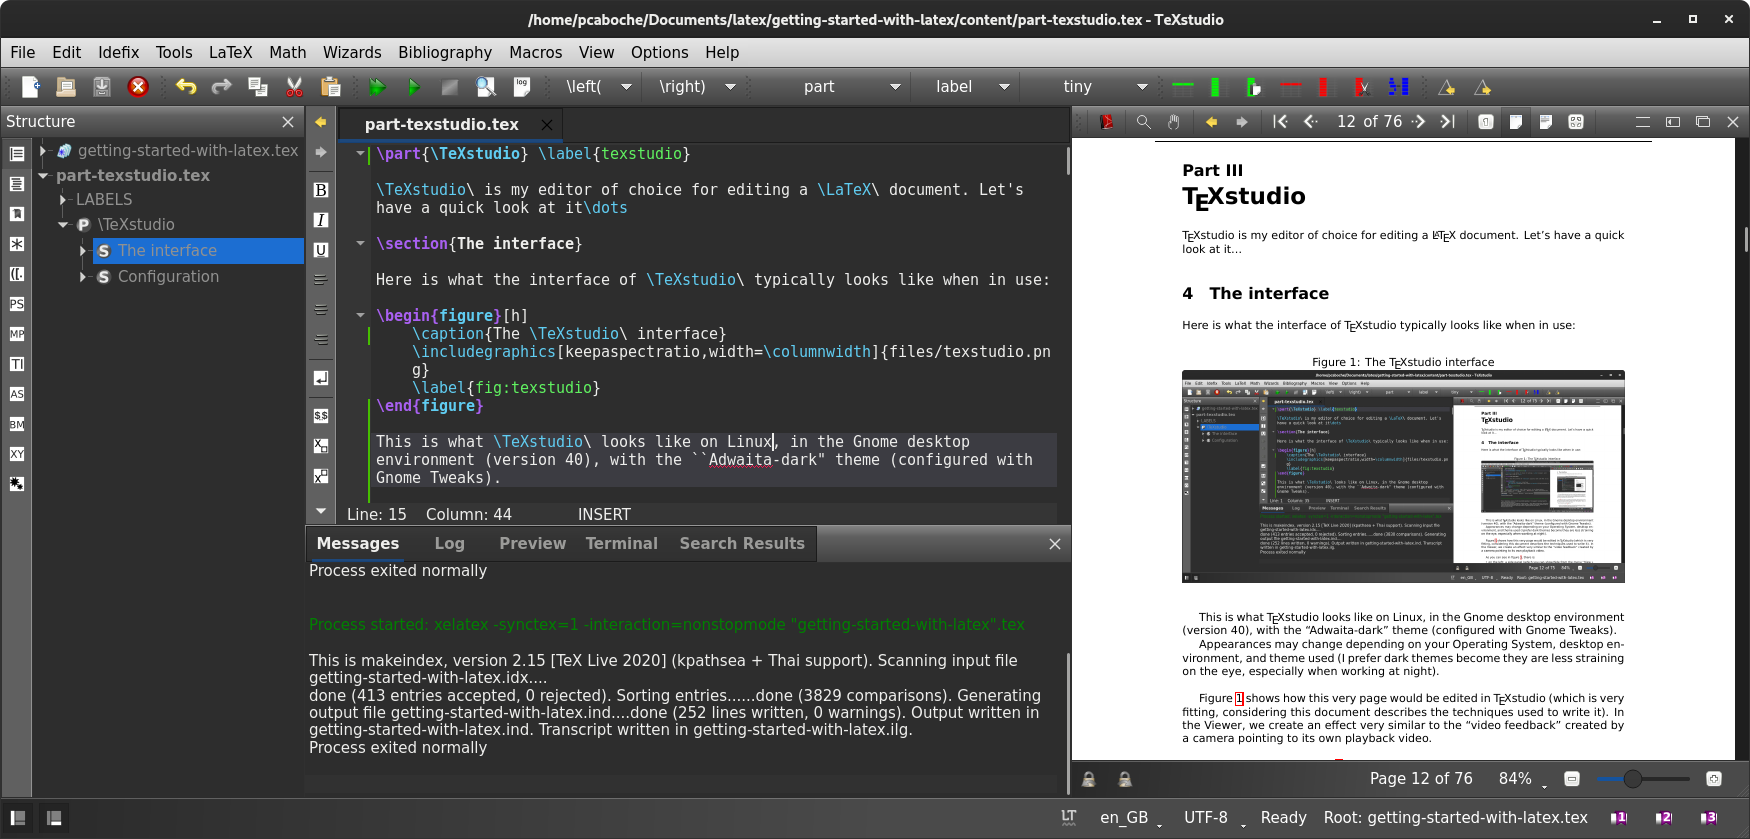
\includegraphics[keepaspectratio,width=\columnwidth]{files/texstudio.png}
	\label{fig:texstudio}
\end{figure}

This is what \TeXstudio\ looks like on Linux, in the Gnome desktop environment (version 41), with the dark theme configured (I find dark themes less straining on the eyes, especially when writing late at night).

Appearances may change depending on your Operating System, desktop environment, and theme used. \\

Figure \ref{fig:texstudio} shows how this very page would be edited in \TeXstudio\ (which is very fitting, considering this document describes the techniques used to write it). In the Viewer, we create an effect very similar to the ``video feedback" created by a camera pointing to its own playback video. \\

As you can see in figure \ref{fig:texstudio}, there is:
\begin{itemize}
	\item on the left: a side panel (which you can show/hide from the menu ``View >> Show >> Side Panel") that will show you the structure of the document, give you access to some \LaTeX\ commands shortcuts, etc.
	\item in the center: the editor for your \LaTeX\ code. \\
	At the bottom of it, you will find a panel for the messages and logs
	\item on the right: the generated document, which will appear after you generate the document from your \LaTeX\ files, by clicking the ``Build \& View" button (or by pressing F5)
	\begin{figure}[h]
		\caption{The ``Build \& View" button (F5)} \label{fig:build-and-view}
		\centering
		
\includegraphics[keepaspectratio,width=2em]{files/build-and-view.png}
	\end{figure} 
\end{itemize}

\TeXstudio\ is best enjoyed on a fairly wide screen (just like many other code editors, where you often have several views side by side). \\

\bigskip

\subsection{Build \& View, Go to Source} \label{build-and-view}

When in the editor, clicking on the ``Build \& View" button (figure \ref{fig:build-and-view}) will generate the document, and highlight the object corresponding to the code where your cursor was in the editor. \\

Similarly, in the editor, select some code, do a right-click, select the ``Go to PDF" option, and \TeXstudio\ will show you the location of the object in the generated document (based on the position of your cursor, not where you performed your right click). \\

Conversely, in the document viewer, do a right-click on any part of the document, select the ``Go to Source" option, and \TeXstudio\ will open the source file, and place the cursor on the code that generated that part of the document (i.e. where you performed the right click). \\

These options make it very easy to navigate between the \LaTeX\ code and the generated document.



\bigskip

\subsection{Toggle Comments}

In \TeXstudio, it is very easy to comment and uncomment parts of the source code.

\begin{itemize}
	\item select the code you want to comment or uncomment
	\item toggle the comments with the ``Ctrl + T" shortcut
\end{itemize}

We will see the importance of comments in the writing process in section ``\longref{comments}". Notably, you can put as many comments as you want in a \LaTeX\ document, so you don't need to discard any draft idea: just comment them out. You'll remove the comment only when you are sure it is not relevant anymore.

\bigskip


\subsection{Undo, Redo}

Like with many editors, ``Undo" in \TeXstudio\ is performed with the ``Ctrl + Z" shortcut. \\
However, please keep in mind that the shortcut for ``Redo" is ``Ctrl + Shift + Z". \\


\bigskip

\subsection{Code completion}

Like with many source code editors, \TeXstudio\ provides some code completion that is tailored specifically for \LaTeX, for example:
\begin{itemize}
	\item commands \\
	Any string starting with \texttt{\textbackslash} will show you a list of possible commands
	
	\item environments \\
	Any string starting with \texttt{\textbackslash begin\{} will show you a list of possible environments
	
	\item references\\
	Typing \texttt{\textbackslash ref\{}, \texttt{\textbackslash nameref\{}, or \texttt{\textbackslash pageref\{} will show a list of available label (see ``\longref{cross-references}")
	
	\item etc.
\end{itemize}



\bigskip

\subsection{Code highlights}

\TeXstudio\ will highlight:
\begin{itemize}
	\item the syntax
	\item words that may be spelled incorrectly (in red squiggly underline)
	\item words that are repeated within a short distance of each other (in yellow squiggly underline)
	\item duplicate labels (in orange)
	\item references that point to non-existing labels (in green squiggly underline)
	\item etc.
\end{itemize}


\subsection{And so much more!}

If you explore the interface of \TeXstudio, you will see that there are many features to fit the needs of different \LaTeX\ users (to the point that it can be really overwhelming at the beginning). \\

I have decided to focus on a few features: the ones that are most universally used, and the ones that are the most useful, especially at the beginning. % (e.g. being able to see the relation between the code and the generated document, as described in section \ref{build-and-view}, really improves productivity!) 
\\

At the core, the interface of \TeXstudio\ is very straightforward: an editor, a document viewer, the ability to jump between the two (as described in section \ref{build-and-view}, a feature that really improves productivity!), code completion, different types of highlights (syntax, references, typos), etc. The workflow (in which we generate a document from \LaTeX\ code) is quite different from other text processors, but we get used to it fairly rapidly. \\

Now that we have a better understanding of what \TeXstudio\ is, and why this is our editor of choice, our next step will be to install all of the necessary software for editing in \LaTeX\dots

\bigskip

\section{Configuration}


\subsection{Configuring \TeX studio}


Go to ``Option >> Configure TeXstudio\dots". A window appears. \\
Select the ``Build" tab


\begin{figure}[h]
	\caption{\TeXstudio's configuration}
	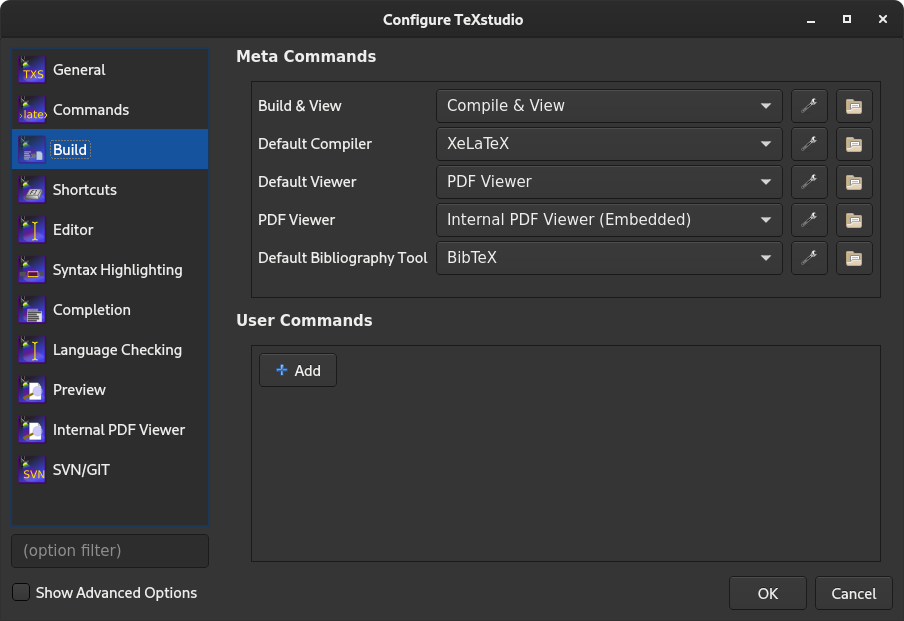
\includegraphics[keepaspectratio,width=\columnwidth]{files/texstudio-configure-embedded.png}
	\label{fig:texstudio-configure-embedded}
\end{figure}


In this screen, we configure the following:

\begin{itemize}
	\item we set ``Default Compiler" to ``XeLaTeX" \\
	This way, we will be able to use the fonts installed on our system
	
	\item we set ``PDF Viewer" to ``Internal PDF Viewer (Embedded)" \\
	This is the default
	
	\item we set ``Default Bibliography Tool" to ``BibTeX" \\
	Needed for section \ref{apa-biblio}
	
\end{itemize}


\subsection{Windowed mode}

There are several reasons why you might prefer to open the PDF Viewer in Windowed mode rather than Embedded mode. For example, your screen might not be wide enough, or you may want to display the PDF Viewer in a secondary screen. \\

Here is how to configure the PDF Viewer in Windowed mode (this setting will apply even after you restart \TeXstudio):

\begin{itemize}
	\item Go to ``Option >> Configure TeXstudio\dots". A window appears. \\ 
	Select the ``Build" tab, then set ``PDF Viewer" to ``Internal PDF Viewer (Windowed)", as shown in figure \ref{fig:texstudio-configure-windowed}
	
	\item If the PDF Viewer is already opened, then close it
	
	\item Press the ``Build \& View" button (figure \ref{fig:build-and-view}), and the ``PDF Viewer" will open in Windowed mode
\end{itemize}




\begin{figure}[h]
	\caption{Setting up \TeXstudio's Viewer in Windowed mode}
	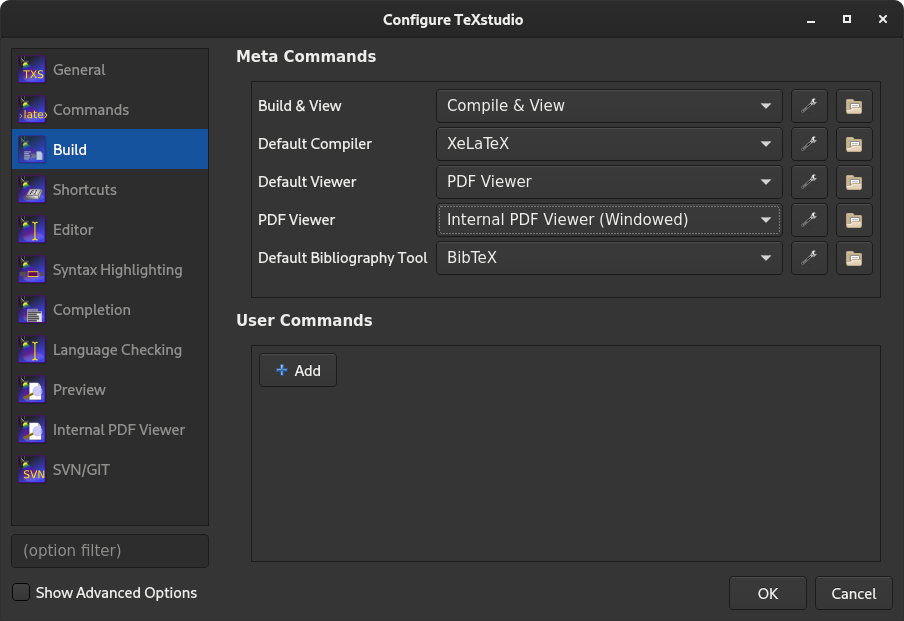
\includegraphics[keepaspectratio,width=\columnwidth]{files/texstudio-configure-windowed.png}
	\label{fig:texstudio-configure-windowed}
\end{figure}


If the PDF Viewer was already in Embedded mode and you want to put it Windowed mode, then press the button highlighted in figure \ref{fig:windowed-viewer} (note that this will not save the setting for after you restart \TeXstudio)

\begin{figure}[h]
	\caption{Windowed Viewer}
	\centering
	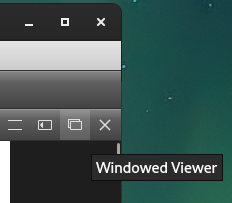
\includegraphics[keepaspectratio,width=6cm]{files/Windowed-Viewer.png}
	\label{fig:windowed-viewer}
\end{figure}





\newpage
%%%%
%% Copyright 2022 Pierre S. Caboche
%% All rights reserved
%%%%

\part{Installation}


\section*{Setting up a \LaTeX\ environment}

The official \LaTeX\ Project website %\citep{latex-project} 
provides some information about \LaTeX\ (including how to install \LaTeX). \\

Link: \url{https://www.latex-project.org} \\

That being said, here is some information to get you started\dots


\subsection*{Windows}

On Windows, I would recommend using \MiKTeX, which includes (among other things):

\begin{itemize}
	\item an \emph{``integrated package manager"}, which will help you download the missing \TeX\ packages, as you need them. This allows you to keep \emph{``just enough \TeX"} on your computer for your work \citep{miktex-project}
	\item \TeXworks, a \emph{``simple \TeX\ front-end program (working environment)"} \citep{texworks}
\end{itemize}

When it comes to \TeX\ editors, I have a preference for \TeXstudio, which we've introduced in \emph{Part \longref{texstudio}} \\



So on Windows, I would usually install the following:
\begin{itemize}
	\item \MiKTeX:   \url{https://miktex.org}
	\item \TeXstudio: \url{https://www.texstudio.org} 
\end{itemize}


\subsection*{Linux}

Under Linux, I tend to install \texttt{texlive}  
(as most Linux distribution provide it through their official repositories, %\citep{texlive})
 as well as an editor for \TeX\ (usually \TeXstudio).

\begin{description}
	\item[texlive] \mbox{} \\ 
	\emph{Required} \\
	\TeX\ formatting system
	
	\item[texstudio] \mbox{} \\
	\emph{Optional, but highly recommended} \\
	A feature-rich editor for \LaTeX\ documents \\
\end{description}


To install these packages in Fedora (requires \emph{super user} privileges):
\begin{lstlisting}[language=sh]
	$ sudo dnf install texlive texstudio
\end{lstlisting}

\bigskip

Additional \TeX\ packages need to be installed separately. \\

Such packages normally have a name that starts with "\texttt{texlive-}" \\
( e.g. \texttt{texlive-mdframed} )

\bigskip



\newpage

%%%%
%% Copyright 2022 Pierre S. Caboche
%% All rights reserved
%%%%

\part{Your first document} \label{your-first-document}


In this article, we will start with an empty document (created from a built-in template), and then slowly add features to it\dots \\

At first, we will focus on the features necessary to add \emph{content} to our document (organising the document, add notes, table of contents, references, cross-references, bibliography, etc), in other words: everything that is important to present inter-connected ideas in a coherent manner. \\

We'll learn how to customise the style later (and if you've been given a template to follow, then you'll not even need to modify the style\dots)


\section{Starting with a template}

In \TeXstudio, go to ``File >> New From Template\dots", select ``Article" in the list of ``Builtin" template, and finally click ``OK". \\

What we get is the following file:
\lstinputlisting[language=tex]{files/empty-article.tex}

Now in \TeXstudio, click on the ``Build \& View" button. This should generate the document without error\dots

\begin{note}
Congratulations! If the document displayed, then you have a working \LaTeX\ environment!\\

With the installation done, we can now concentrate on learning \LaTeX\ itself. (note: you might still need to install additional packages when required)
\end{note}

\bigskip

Let's take a look at that file\dots \\

A \LaTeX\ file has two main parts:
\begin{itemize}
	\item the \emph{preamble} (everything before \lstinline[language=tex]|\begin{document}| ), which the template calls \emph{``opening"}
		
	\item the document's \emph{body} (\lstinline[language=tex]|\begin{document}| and all of its content)
\end{itemize}

\medskip

The \emph{preamble} is where we invoke all the packages necessary to generate our documents, as well as configure those packages. Some \LaTeX\ commands can only be called in the \emph{preamble} (they will throw an error if called in the \emph{body}); this is especially the case with configuration commands). \\

The \emph{body} is where our document's content goes. \\

\medskip

The \quoteCmd{documentclass} command specifies which document class (template) our document follows. We chose the class \texttt{article}, but there are others built-in in \LaTeX\ (\texttt{letter}, \texttt{beamer}, \texttt{book}, \texttt{memoir}\dots). 

The square brackets \texttt{[]} is where we specify options to our document class, for example \texttt{twoside} %to indicate that each page is to be printed on two sides, and then bound together 
(section \ref{two-sided}). \\

In the \emph{preamble} of our template, you can notice the following commands: \quoteCmd{title} and \quoteCmd{author}. As the name implies, their goal is to declare the document's title and author (section  \ref{set-title-author}).

Then in the \emph{body}, the command \quoteCmd{maketitle} generate the document's title (including author, as well as date). It is possible to  customise the date (section \ref{customise-date}). \\

We'll examine the rest of the template in the following sections:
\begin{itemize}
	\item \lstinline[language=tex]|\begin{abstract}|: section \ref{write-abstract}
	\item \lstinline[language=tex]|\section{}|: section \ref{parts-sections}
\end{itemize}

\bigskip

\subsection{Set the title and author} \label{set-title-author}

The first thing we'll do to that template document, is specify the title and author, which is really straightforward:
\begin{lstlisting}[language=tex]
\title{Article title}
\author{Your Name here}
\end{lstlisting}

\idxCmd{title}
\idxCmd{author}

Next we will modify the document's date\dots 

\subsection{Customise the date}  \label{customise-date}

By default, \quoteCmd{maketitle} will print out the date the document has been last generated (the result of calling \quoteCmd{today}), but we might want to change this for different reasons\dots \\

One reason could be that we want to specify a publication date, and not change afterwards.

Another reason would be to add a revision date, on top of the publication date that is set in stone. We are going to do the latter. \\

Here is how we do it, using the \quoteCmd{date} command:
\lstinputlisting[language=tex]{include/featured/pkg-custom-date.tex}




\newpage

\subsection{Write an abstract} \label{write-abstract}

In our ``Article" document template, you will notice the following block:

\begin{lstlisting}[language=tex]
\begin{abstract}
	
\end{abstract}
\end{lstlisting}

\idxEnv{abstract}

As the name implies, this is where you need to write the abstract for your article. \index{abstract} \\

\bigskip

An abstract is the summary of a research paper (whether published or not). The goals of an abstract is to:
\begin{itemize}
	\item introduce the content of the paper
	\item present some of the ideas developed in the paper
	\item help remember the key points
\end{itemize}

\medskip

An abstract is usually short (one paragraph, 6-7 sentences, 150-200 words). \\


\medskip


If you don't know what to put in an abstract, then a good tip I was given years ago was to
write one or two sentences for each of the following subjects:

\begin{center}
\textbf{B}ackground, \textbf{P}urpose, \textbf{M}ethodology, \textbf{R}esults, \textbf{C}onclusion 
\end{center}

Usually: 1 sentence per subject, and an extra sentence each for Methodology and Conclusion. \\


So that's what the ``abstract" is\dots\ I know, this has nothing to do with \LaTeX, but people might be wondering about the purpose of this block. \\
\medskip

Note that I don't always follow those rules for my articles. Specifically, my abstracts tend to be longer and describe the paper in more details.

\bigskip


\section{Organising your files} \label{getting-organised}


\subsection{File hierarchy}

Unlike other text editors (e.g. LibreOffice), a \LaTeX\ document can be made up of multiple files.

On top of that, \LaTeX\ will create a number of other intermediate files (with extensions such as: \texttt{.aux}, \texttt{.bbl}, \texttt{.blg}, \texttt{.idx}, \texttt{.ilg}, \texttt{.ind}, \texttt{.lof}, \texttt{.log}, \texttt{.log}, \texttt{.out}, \texttt{.toc}, and even a \texttt{.gz} archive), as well as the final \texttt{.pdf} file. \\

All these files will be found in the same folder (in addition to \emph{our} own files, which will define the content of our document). So we need to organise this folder. \\

Our goal is to have only one \texttt{.tex} file at the root of our folder hierarchy, and all other files grouped in different folders. \\

Here is the main hierarchy that I used for this document\footnote{folders may contain sub-folders}:
\begin{description}
	\item[\texttt{include/}] \mbox{} \\
	folder contains our external dependencies, configurations, and custom macros.
	In particular:
	\begin{description}
		\item[\texttt{packages.tex}] \mbox{} \\
		file containing all our dependencies and their configuration
		\item[\texttt{macros.tex}] \mbox{} \\
		file containing our custom macros.
	\end{description}

	\item[\texttt{content/}] \mbox{} \\
	folder containing all the \texttt{.tex} files that form the content of our article,
	divided in parts / chapters / sections, etc.
	
	We also use this folder to store bibliography files (\texttt{.bib}), see Section \ref{add-biblio} \\
	
	I also strongly suggest that you organise your files in a way that makes it easy to see if they belong to a part / chapter / section or other. One way to achieve this is by adopting some naming conventions for your files. \\
	
	For example:
	\begin{description}
	\item[] \mbox{} \\
		\texttt{part-(...).tex\\
		chapter-(...).tex\\
		section-(...).tex}
	\end{description}


	\item[\texttt{files/}] \mbox{} \\
	folder containing other files necessary for generating the document (e.g. images, source code files\dots)
\end{description}

\begin{note}
You are free to use whichever file structure you want. However, in this article we will be using the structure described above, and will refer to each folder or file by their name in that hierarchy.
\end{note}


\bigskip


For your \LaTeX\ documents, I suggest that you organise your files sooner rather than later: \\

Starting from a template, you may start adding the different parts, sections, sub-sections 
(section \ref{parts-sections}) to lay out the structure of your document. 
Then you may add a Table of Content (section \ref{add-toc}) to better see that structure.

Finally, in the different sections you may add some notes in the form of comments (see ``\longref{comments}") to know which ideas will go into which section. \\

At that point, you may still have most of your ideas in just one \LaTeX\ file. \\

However, when you start writing the actual content of your document (not just adding sections names and comments), that's when you need to make different files (in the \texttt{content/} folder).


\newpage

\subsection{Using \texttt{\textbackslash input}}

The \quoteCmd{input} command is used to load the content of a file, \emph{verbatim}, into the current document, where the \quoteCmd{input} command has been called.

\begin{lstlisting}[language=tex]
%% Importing our custom macros
% Copyright 2022 Pierre S. Caboche. All rights reserved.

\usepackage{mdframed}
\mdfsetup{
	%innertopmargin=10pt,
	frametitleaboveskip=-\ht\strutbox,
	frametitlealignment=\center
}


\newcommand{\note}[1]{
	\mdfsetup{
		middlelinewidth=2pt,
		backgroundcolor=yellow!10
	}
	\begin{mdframed}#1\end{mdframed}
	\mdfsetup{
		backgroundcolor=white
	}
}


\newcommand{\cmd}[1]{\lstinline|#1|}


\newcommand{\python}{Python}
\newcommand{\awk}{AWK}
\newcommand{\perl}{Perl}
\newcommand{\julia}{Julia}
\newcommand{\gawk}{\texttt{gawk}}
\newcommand{\mawk}{\texttt{mawk}}
\newcommand{\sed}{\texttt{sed}}
\newcommand{\grep}{\texttt{grep}}

\newcommand{\stdin}{\texttt{stdin}}
\newcommand{\stdout}{\texttt{stdout}}
\newcommand{\stderr}{\texttt{stderr}}

\newcommand{\mysqldump}{\texttt{mysqldump}}
\newcommand{\cat}{\texttt{cat}}
\newcommand{\pv}{\texttt{pv}}
\newcommand{\shell}{\texttt{shell}}

\newcommand{\Unix}{UNIX\textregistered}
\newcommand{\Intel}{Intel\textregistered}
\newcommand{\Core}{Core\texttrademark}



  ...

%% Adding some content to our document
%%%%
%% Copyright 2022 Pierre S. Caboche
%% All rights reserved
%%%%

\part{Text styles, indexes}

In this part, we'll talk about custom text styles and adding indexes.  
This will be useful when we learn how to write our first macros, in section ``\longref{first-custom-macro}".

\section{\emph{Emphasis}, italics, bold\dots} \label{text-style}

A recurring question from people new to \LaTeX\ is: \emph{``how do I put text in \textbf{bold} face?"} when the underlying question really is \emph{``how can I \emph{emphasise} some important idea?"} \\

In \LaTeX, there is a command specifically used for \emph{emphasis}: \quoteCmd{emph}

The difference is, by default in \LaTeX, \emph{emphasis} is not made using \textbf{bold face}, but using \textit{italics} instead.

Also, \emph{if you were to \emph{emphasise} some text inside of another \emph{emphasis}, then the inner \emph{emphasis} will appear \emph{upright} (and not in italics), as if the two \emph{emphases} had cancelled each other\dots} \\

So we advise you to \quoteCmd{emph} for emphasis in \LaTeX. \\

However, if you really \emph{must} specifically put your text in bold, italics, underline, etc., then here are some commands for that: \\

\begin{tabular}{l l l l}
	\quoteCmd{emph}\texttt{\{text\}}      & \emph{text}      & \emph{emphasis}          \\
	\quoteCmd{textit}\texttt{\{text\}}    & \textit{text}    & \textit{italics}         \\
	\quoteCmd{textbf}\texttt{\{text\}}    & \textbf{text}    & \textbf{bold face}       \\
	\quoteCmd{texttt}\texttt{\{text\}}    & \texttt{text}    & \texttt{monospaced font} & \footnotesize (as configured in section \ref{changing-the-fonts}) \\
	\quoteCmd{underline}\texttt{\{text\}} & \underline{text} & \underline{underlined}   \\
\end{tabular}


\section{Adding an index} \label{add-index}

First, we need to use the \quotePkg{imakeidx} package and call the \quoteCmd{makeindex} command:

\lstinputlisting[language=tex]{include/featured/pkg-imakeidx.tex} 

Then we need to use the \quoteCmd{index} command, to add an index on the relevant word:

\begin{lstlisting}[language=tex]
Some text here, mentioning a keyword to be indexed. \index{keyword}
\end{lstlisting}


Finally, we need to print the index with \quoteCmd{printindex} :

\begin{lstlisting}[language=tex]
\printindex
\end{lstlisting}

The difficult part is to specify an index whenever certain words are mentioned.
For this purpose, we can use macros to make our task easier\ldots \\

To see what an index looks like, go to page \pageref{our-index} (for this is where you will find the index for this document).


\end{lstlisting}

\bigskip

This way, the content of our document can be broken down into smaller, more manageable files, but they will appear as one big file to the \LaTeX\ compiler. As a result of this behaviour\dots

\begin{note}
The path specified as parameter to the \quoteCmd{input} command 
is always relative our main \texttt{.tex} document at the \emph{base} of our folder hierarchy.
\end{note}

For example, if from a \texttt{.tex} document in our \texttt{content/} folder we include another \texttt{.tex} file, its path must be relative to the \emph{base} of our folder hierarchy, where our main \texttt{.tex} document is located.

\begin{note}
This is also true for other \LaTeX\ command that accept a file path as a parameter, like \quoteCmd{includegraphics} (page \pageref{includegraphics}), or \quoteCmd{lstinputlisting} (page \pageref{lstinputlisting}).
\end{note}

\bigskip

The \quoteCmd{input} command is not to be confused with the \quoteCmd{usepackage} command\dots\
(see next section) \\


\subsection{Calling \texttt{\textbackslash usepackage}}
The \quoteCmd{usepackage} command is used to load one or more \LaTeX\ packages, sometimes with some parameters. \\

For example:
\begin{lstlisting}[language=tex]
%%% In the preamble
	
%% Loading one package
\usepackage{xstring}

%% Loading several packages
\usepackage{titleps, xcolor}

%% Loading one package, with some option
\usepackage[super]{nth}
\usepackage[authoryear]{natbib}
\end{lstlisting}

Note that \quoteCmd{usepackage} can only be called in the preamble (not in the body of the document).

\newpage
\section{Parts, Sections, etc.} \label{parts-sections}

A document of class \texttt{article} (like this one), is divided into: parts, sections, subsections. 
The document class \texttt{book} also adds the ``chapter" subdivision: \\

\quoteCmd{part}

\quoteCmd{chapter} (\texttt{book} only)

\quoteCmd{section}

\quoteCmd{subsection} \\


For example:
\begin{lstlisting}
\part{Your first document}
   % ... introduce the part ...
   
\section{Starting with a template}
   % ... content of the section ...

\subsection{Set the title and author}
   % ... content of the subsection ...
\end{lstlisting} 

\bigskip

The previous commands will define the different subdivisions that need to be \emph{numbered}.
Such subdivisions will not only be assigned a number, but they will also appear in the Table of Contents if you add one (see Section \ref{add-toc}). \\

Also worth noting: the \quoteCmd{part} command does not reset the numbering of the chapters / sections it contains (i.e. you could have Sections 1, 2, 3 in part I; Sections 4, 5, 6, 7 in part II, etc.)

\bigskip

If you don't want to number a subdivision, use the \emph{starred} version of the previous commands, i.e.:

\quoteCmd{part*}

\quoteCmd{chapter*} (\texttt{book} only)

\quoteCmd{section*}

\quoteCmd{subsection*} \\


\begin{note}
Non-numbered subdivisions will not appear in the Table of Contents.
\end{note}


\newpage

\section{Adding a Table of Contents (TOC)} \label{add-toc}

Adding a table of contents is very easy. \\

Just call \quoteCmd{tableofcontents} where you want your Table of Contents to be (only one per document) :
\begin{lstlisting}[language=tex]
\tableofcontents
\end{lstlisting}



\subsection{Customising the Table of Contents} \label{customising-toc}

It is also possible to customise the Table of Contents. \\

Here is what I used for this article:
\lstinputlisting[language=tex]{include/featured/customise-toc.tex}

\bigskip

\begin{note} 
Note: if you modify those parameters, you might need to generate your document several times for the changes to take effect.
\end{note}

\bigskip

More customisation options can be found at \citep{customize-toc} : \\

\hfill
\url{https://texblog.org/2011/09/09/10-ways-to-customize-tocloflot/}


\bigskip	


%%%%
%% Copyright 2022 Pierre S. Caboche
%% All rights reserved
%%%%


\newpage

\section{Paragraphs, footnotes}

In this section, we will learn how to make paragraphs, sub-paragraphs, etc. \\

The best way to explain how it works is to show the \LaTeX\ code, and show you how it renders. \\



This is the \LaTeX\ code:

\lstinputlisting[language=tex]{content/sample-paragraphs.tex}

\bigskip



\dots and this is the output. Please note that the code explains how paragraphs work. I needed some sample text, but instead of using a generic \LoremIpsum, I figured that this section could be self-describing\dots

\bigskip

\begin{mdframed}
	This is the first line of our first paragraph (after all, we have to start somewhere\ldots)
This is on a new line (in the \LaTeX\ code), but it is still part of the same paragraph (in the generated document); so it is possible to add comments without disrupting the flow of the paragraph. For example\dots\ 
% This is a comment...
% Everything after the % until the end of the line is a comment, and will be ignored
this was added after the comment. As you can see, this is still part of the same paragraph; the comment didn't appear, and the flow of text was not disrupted.


By leaving (at least) one empty line between this and the previous block of text, we start a new sub-paragraph. Sub-paragraphs are very useful if you want to introduce a new topic in continuation with the previous point, but not a completely new idea that would warrant a new paragraph.

If you want to create a new paragraph, you need to terminate the current paragraph with a pair of backslashes ( \texttt{\textbackslash\textbackslash} ) and then leave at least one empty line between this and the next block of text.
\\


This is the start of a new paragraph. Now let's see what happens when we add a pair of backslashes ( \texttt{\textbackslash\textbackslash} ) but do not leave an empty line with the next block of text\dots 
\\
This is a new sub-paragraph; but unlike the others, this one is not indented (please, bear in mind: in some cases, that can make it difficult to see that this is a sub-paragraph at all).
\\

So far we've seen that a new paragraph can be used to introduce a new idea, while a new sub-paragraph can be used to introduce a new point pertaining to the same idea. The layout of the text (indentation, line breaks) will help us differentiate the different ideas/points.
\\

\medskip

And if you need a bigger break between paragraphs, you can use \texttt{\textbackslash medskip} or \texttt{\textbackslash bigskip} (medium or big skip, respectively). Use sparingly, though.

\begin{center}
	\textreferencemark\textreferencemark\ 
	Now, a word about footnotes\dots\ 
	\textreferencemark\textreferencemark
\end{center}

Sometimes when talking about a particular subject, you might feel the need to add some related information. Your first instinct would be to put such information in parentheses (but the problem with parentheses is that they appear in the middle of a text, and break the flow of the discussion. So you usually want to keep them both short and relevant. This is a counter-example, to illustrate what happens when the content in parentheses is too long: we tend to lose focus and forget what we were talking about). \\

One way to avoid being side-tracked by tangent ideas is to use \emph{footnotes}. As the name implies, footnotes are notes that appear at the foot of the page (or, in this case, at the end of a \texttt{mdframed} box) and referred to by number, like this\footnote{this is an example of a footnote. A footnote will not disrupt the flow of the discussion, so they can be used to add some comment or extra information that would be too long to put in parentheses
}.\\
\end{mdframed}


\bigskip
\bigskip


\subsection{Footnotes} \label{footnote}

In the previous code sample, we saw an example of a \texttt{footnote}. \\

In \LaTeX, it's very easy to add a footnote with the \lstinline[]|\footnote| command:
\begin{lstlisting}[language=tex]
This is some text\footnote{and this is the footnote}.
\end{lstlisting}
\medskip

Footnotes will appear at the foot of the page (see: example\footnote{this is an example of a footnote. As you can see, it is able to hold a lot more information than a margin note
}), 
or at the bottom of components like a \texttt{mdframed} box. \\

As mentioned earlier, footnotes can be useful when you want to add some information but it would be too long to put in parentheses without disturbing the flow of ideas.\\

\bigskip

So the following can be used to add additional information:
\begin{itemize}
	\item parentheses: used for short explanations, closely related to the subject
	\item footnotes: used for additional information that is either too long to be in parentheses, or not closely related to the subject
	\item margin notes (section \ref{margin-notes}): to bring the reader's attention on a particular subject
\end{itemize}

\newpage


\subsection{Margin notes and paragraphs} \label{margin-notes}

\LaTeX\ also allows to put notes in the margins, thanks to \emph{margin paragraph} and \emph{margin notes}.
\\

\idxCmd{marginpar}
\marginpar{This is a margin paragraph} To 
add a margin paragraph, use the \lstinline[language=tex]|\marginpar| 
command:
\lstinputlisting[language=tex]{content/sample-marginpar.tex}


\medskip

To add a \emph{margin note}, you will need \quotePkg{marginnote} package, 
which provides the \quotePkg{marginnote} command:
\lstinputlisting[language=tex]{include/featured/pkg-marginnote.tex}
\medskip

\idxCmd{marginnote}
\marginnote{This is a margin note} A 
margin note can be added by using the \lstinline[language=tex]|\marginnote| 
command:
\lstinputlisting[language=tex]{content/sample-marginnote.tex}


\bigskip

Notice how in both cases, we put the \quotePkg{marginpar} or \quotePkg{marginnote} command immediately after the first word in the paragraph. This is to make sure the margin paragraph/note will be aligned vertically with the first word of the paragraph. \\

Also keep in mind that in a two-sided document (section~\ref{two-sided}), a margin paragraph will be on the \emph{outer} margin (i.e. left margin for even-numbered pages, right margin for odd-numbered pages). If the document is one-sided, margin paragraphs will appear in the right margin. \\


A \marginpar{marginpar vs. \\ footnote}
margin paragraph (or note) stands out from the rest of the text. 
They can be used to bring the reader's attention on a particular paragraph. However, \emph{it is better to keep them short}. \\

In contrast, a footnote (\emph{section \ref{footnote}}) can be much longer, and is used to provide additional information without breaking the flow of the discussion.
\newpage



\subsection{Putting text in a frame} \label{mdframed}

Previously, we've seen how margin notes and margin paragraphs could be used to bring attention to certain parts of your document. \\

Now we will learn how to make some ideas stand out, by putting them in a big box, thanks to the \quotePkg{mdframed} package:
\lstinputlisting[language=tex]{include/featured/pkg-mdframed.tex}

\bigskip

The \quotePkg{mdframed} package defines, amongst other things, the \quoteEnv{mdframed} environment. Here is a very simple example :
\lstinputlisting[language=tex]{include/featured/example-frame-1.tex}

You can notice how an environment is delimited by \texttt{\textbackslash begin\{\emph{envname}\}} and \\
\texttt{\textbackslash end\{\emph{envname}\}}. \\

And here is the result of the code above:
\begin{mdframed}
Help! I've been framed!
\end{mdframed}



\bigskip



This is a very simple frame, but we can modify its appearance with the \quoteCmd{mdfsetup} command.

One thing to know about the \quoteCmd{mdfsetup} command, is that is modifies the properties of \emph{every} \quoteEnv{mdframed} that comes after it. This is a problem if you want to modify the attributes of only \emph{one} frame. \\


To get around this issue, we will create an \emph{environment}. \\
We will name it ``\texttt{vegas}". Why? because \emph{``what happens in \emph{\texttt{vegas}} stays in \emph{\texttt{vegas}}"} (and what happens in an environment stays in that environment"). \\

So here is our ``\texttt{vegas}" environment:
\lstinputlisting[language=tex]{include/featured/example-frame-vegas-env.tex}
\newenvironment{vegas}[1][!!! Welcome to Vegas !!!]{
	\mdfsetup{
		frametitle={
			\tikz
			\node[rectangle,fill=yellow!60,draw=red, ultra thick]
			{#1};
		},
		frametitleaboveskip=-\ht\strutbox,
		frametitlealignment=\centering,
		backgroundcolor=yellow!30,		
		linewidth=4pt,
		linecolor=red!70,
		roundcorner=8pt,		
		shadow=true,
		shadowcolor=orange!40,
	}
	\begin{mdframed}}
	{\end{mdframed}}


For the purpose of this example, we declared this environment with one optional parameter: the title of the frame, which defaults to ``!!! Welcome to Vegas !!!". \\

Now it's time to use this environment:
\lstinputlisting[language=tex]{include/featured/example-frame-vegas.tex}

And here is what it looks like: \\
\begin{vegas}
What happens in this environment stays in this environment\ldots
\end{vegas}


\bigskip

Wow, so many colours! \\


\bigskip

Now, let's create another frame:
\lstinputlisting[language=tex]{include/featured/example-frame-2.tex}

And here is the result:
\begin{mdframed}[
	frametitle={The title of the frame},
	frametitleaboveskip=-\ht\strutbox,
]
Help! I've been framed!
\end{mdframed}



As you can see, our very flamboyant ``\texttt{vegas}" environment did not have any influence over to the new frame. The \quoteCmd{mdfsetup} command only affected the environment where it was used (i.e. ``\texttt{vegas}"), and had no effect outside of it. \\

\bigskip


Again, we can define a new environment, call \quoteCmd{mdfsetup} inside of it, and the effect of \quoteCmd{mdfsetup} will not be seen outside of the environment:
\lstinputlisting[language=tex]{include/featured/example-frame-blue-env.tex}
\newenvironment{blueframe}[1]{
\mdfsetup{
	frametitle={
		\tikz
		\node[rectangle,fill=blue!20]
		{#1};
	},
	linecolor=blue!20,
	linewidth=2pt
}
\begin{mdframed}}
{\end{mdframed}}



\lstinputlisting[language=tex]{include/featured/example-frame-blue.tex}


Result:
\begin{blueframe}{Put title here}
Help! I've been framed!
\end{blueframe}



\bigskip

In our two previous environments (``\texttt{vegas}" and ``\texttt{blueframe}"), we passed the frame title as a parameter (whether optional or mandatory). However, if we don't need to add a title, there is a simpler way to define frame environment, thanks to the \quoteCmd{newmdenv} command. \\


Below is the definition for ``\texttt{note}", an environment which I used to add some important notes throughout this document, in the form of a frame with a slightly yellow background:
\lstinputlisting[language=tex]{include/featured/note-env.tex}

Here is how to call it:
\lstinputlisting[language=tex]{include/featured/example-frame-note.tex}
Here is the result:
\begin{note}
This is an example of note.
\end{note}



\bigskip

As you can see, all the options that we would normally pass to the \quoteCmd{mdfsetup} command are passed in the optional parameter (in square brackets \texttt{[]}) of \quoteCmd{newmdenv}. \\
The name of the environment is passed as the mandatory argument (in curly brackets \texttt{\{\}}) of \quoteCmd{newmdenv}.

\bigskip

Another way to modify the appearance of a \quoteEnv{mdframed} is to define a new style with the \quoteCmd{mdfdefinestyle} command, then use that style by specifying the \texttt{style} attribute in the \quoteEnv{mdframed} options:

\lstinputlisting[language=tex]{include/featured/example-frame-pinky-env.tex}
And the result:
\mdfdefinestyle{pinky}{
	linecolor=pink,
	linewidth=2pt,
	backgroundcolor=pink!30
}

\begin{mdframed}[style=pinky]
They're Pinky and the Brain, \\
Yes, Pinky and the Brain, \\
One is a genius, the other's insane\ldots
\end{mdframed}



\bigskip


This concludes our presentation of \quotePkg{mdframed}. \\

If you want to know more about this package (with many other examples), please refer to its official documentation: 
\begin{center}
\url{https://www.ctan.org/pkg/mdframed}
\end{center}


\newpage

\subsection{Other types of boxes}

There exists other kinds of boxes, to draw boxes around text:
\begin{itemize}
	\setlength{\itemsep}{-0.5em}
	
	\item \quoteCmd{parbox}
	\item \quoteCmd{mbox}
	\item \quoteCmd{makebox}
	\item \quoteCmd{fbox}
	\item \quoteCmd{framebox}
	\item \quotePkg{fancybox} (package)
\end{itemize}

\bigskip

For more information, please see:
\begin{center}
	\url{https://en.m.wikibooks.org/wiki/LaTeX/Boxes}
\end{center}

\bigskip



\section{Comments} \label{comments}


In \LaTeX, a comment starts with: \% \\


Everything after the ``\%" till the end of the line will be ignored. If you want to actually print a ``\%" in \LaTeX, you'll need to escape it with a backslash: \textbackslash \% \\

Unlike in other computer languages, there are no multiline comments in \LaTeX, only single-line comments.
\\


Fortunately, an editor like TeXStudio can make the process of adding/removing comments a lot easier, thanks to the \texttt{Ctrl+T} shortcut (for \emph{``Toggle Comment"}).

\begin{mdframed}
\medskip
	To toggle comments in TeXStudio:
	\begin{itemize}
		\item Select the lines you want to add comments to (or remove comments from)
		\item Press \texttt{Ctrl+T}
		
		This will either add or remove the comments from those lines
	\end{itemize}
\medskip
\end{mdframed}



Comments are extremely useful in \LaTeX! In fact\dots 

\begin{note}
When you think about it, comments are one of the most powerful features in \LaTeX. \\

Indeed, comments allow you to keep multiple drafts of the same paragraphs, which you can then enable/disable with a single \texttt{Ctrl+T} in \TeXstudio. This way, you never have to throw away any idea! (just comment them out, so they don't show up in the document).
\end{note}



Comments have a number of applications:

\begin{description}
	\item[\emph{Describing}] \mbox{}\\
	The most obvious use of a comment is to describe what some \LaTeX\ code is doing (e.g. describe the packages that you are using and what you are using them for)
	
	\item[\emph{Taking notes}] \mbox{}\\
	For example, if you already have your document's plan laid out (i.e. you've already defined the structure in terms of: parts, sections, sub-sections\ldots), you can leave comments to list the main ideas to put in those sections later (as some kind of \emph{TODO} list)
	
	Furthermore, if several people are working on a document you can leave notes to other contributors in the form of comments (and if you work alone, you can always leave notes to yourself)
	
	\item[\emph{Drafting ideas}] \mbox{}\\
	This is probably the most important use of comments (this represents about 99\% of the cases when I use comments in \LaTeX)
	
	Sometimes you're writing things but are not completely satisfied with the wording. In \LaTeX, it's very easy to put a sentence in comments, rewrite it, and repeat the process until you're satisfied (while not having to discard what you wrote, and not having those earlier versions appear in your document).
\end{description}


In many of those cases, you don't want your comments to be removed by accident (i.e. any case other than \emph{Drafting ideas}). To avoid that, simple use more than one ` \lstinline|%| ' for your comment. \\

This way, one \texttt{Ctrl+T} will not be enough to remove the comment\ldots
\begin{lstlisting}[language=tex]
%%% Packages and configuration
\end{lstlisting}


\bigskip


\section{Collaboration, version management}

The main focus of \LaTeX\ is document generation. As such, it does not provide dedicated collaboration and version management tools. \\

However, \LaTeX\ is a markup language. This means that, collaboration and management of \LaTeX\ files can be handled with the same tools as any other source files; so you can use your favourite version management tools with \LaTeX\ (e.g. GIT, SVN\dots) \\

In section ``\longref{comments}", we've seen how \LaTeX\ comments can be used for note-taking, drafting entire paragraphs, etc. A version-control management system can help you keep a history of such items.


\newpage

\part{Managing breaks}

In part \ref{your-first-document}, we talked about how to how to write paragraphs, how to organise your documents in sections, etc. \\

Sometimes, however, a paragraph or section break does not land in a place that is convenient for us, as it disrupts the flow of the article, For example, a section may start at the bottom of a page, a figure may end up on a different page from the text that references it (I always find this confusing to read when that happens), etc. 

To avoid that, you might want to make some manual adjustments to the document layout. This is the subject of this part\dots

\section{Non-breaking spaces}

In \LaTeX, you can create a non-breaking space by using a tilda: $\sim$ \\

Non-breaking spaces are used to keep certain terms together, without automatic line breaks being inserted in the middle. \\

This is useful, for example, to keep numbers and their units together:

\begin{lstlisting}[language=tex]
	The maximum theoretical speed of SATA-3 is 6~Gb/s, or 750~MB/s.
\end{lstlisting}

\medskip

Whenever possible, \LaTeX\ will keep those terms together. \\

In the previous example, the ``6" should not be separated from its ``Gb/s" unit, and the ``750" should not be separated from the ``MB/s".

\bigskip


\section{Phantom text} \label{phantom}

Since we are on the subject of adding breaks and spaces, here are the commands to add some empty space based on the width/height of a given text:

\begin{description}
	\item{\quoteCmd{phantom}\texttt{\{text\}}} \mbox{} \\ 
		Creates some space, of the same width and height as the \texttt{text} passed as parameter
		(a combination of \quoteCmd{hphantom} and \quoteCmd{vphantom})
		
	\item{\quoteCmd{hphantom}\texttt{\{text\}}} \mbox{} \\ 
		Creates some horizontal space, of the same width as the \texttt{text} passed as parameter
	\item{\quoteCmd{vphantom}\texttt{\{text\}}} \mbox{} \\ 
		Creates some vertical space, of the same height as the \texttt{text} passed as parameter
\end{description}

\newpage

Below is an example of how to put an \quoteCmd{underline} under some \quoteCmd{phantom} text:
\begin{lstlisting}[language=tex]
I really think that \underline{\phantom{\LaTeX}} is great!
\end{lstlisting}

And here is the result:
\begin{mdframed}
I really think that \underline{\phantom{\LaTeX}} is great!
\end{mdframed}

\bigskip

\section{Skips and breaks}


\subsection{Adding vertical spaces}

Sometimes you might need to add some extra vertical space between paragraphs (or other elements). These are called ``skip". \\

Skips come in different sizes: \\

\begin{tabular}{l l}
	\quoteCmd{smallskip} & a small skip \\
	\quoteCmd{medskip}   & a medium skip \\
	\quoteCmd{bigskip}   & a big skip \\
\end{tabular}

\bigskip


\subsection{Page breaks}

You can start a new page with the \quoteCmd{newpage} command. \\

You can also start a new page with \quoteCmd{pagebreak}, in which case the content of the old page will be spread out vertically. \\

Having several \quoteCmd{newpage} (or \quoteCmd{pagebreak}) will not create empty pages. To insert empty page(s), see section \ref{blank-page}\dots

\bigskip


\subsection{Inserting a blank page} \label{blank-page}


While writing about \quoteCmd{newpage} and \quoteCmd{pagebreak}, I wondered \emph{``how to insert a blank page in a \LaTeX\ document?"} \\

After a minute of searching, I found the following solution, which I then wrapped in a custom macro with an optional parameter (section \ref{macro-optional-parameter}):


\lstinputlisting[language=tex]{include/featured/cmd-insertBlankPage.tex}


The macro will insert a blank page, with a custom message (passed as an optional parameter) written in the center of the page. If the message is not specified, it will default to ``This page intentionally left blank." \\

This macro uses the \quoteCmd{thispagestyle} command, which sets the style for the current page only. By setting it to \texttt{empty}, we remove the header and footer temporarily. Therefore only the message will appear on the center of the page. \\

Here are some examples of how to call our custom macro:
\begin{lstlisting}[language=tex]
% To display a blank page with a custom message
\insertBlankPage[Some text]

% To display a blank page 
% with the default "This page intentionally blank."
\insertBlankPage

% In this case, the message will actually be blank
\insertBlankPage[]
\end{lstlisting}


\bigskip

We will be calling the following:
\begin{lstlisting}
\insertBlankPage
\end{lstlisting}

See next page for the result\dots
\insertBlankPage









\newpage
%%%%
%% Copyright 2022 Pierre S. Caboche
%% All rights reserved
%%%%

\part{Cross-references, bibliography}


\section{Cross-references} \label{cross-references}

Adding a cross-reference in \LaTeX\ is easy! \\

First, you need to put a label next to the object you want to reference (e.g. section, table, figure\ldots) This is done with the \lstinline|\label| command:

\begin{lstlisting}[language=tex]
\section{Cross-references} \label{cross-references}
\end{lstlisting}

\medskip

Of course, labels must be \emph{unique}! \\

Don't worry though, \TeXstudio\ will highlight any label that has been defined more than once in a document. \\

Labels are \emph{case-sensitive}, but they can be \emph{any} string of characters (including numbers, white spaces, punctuation, multibyte unicode characters\ldots) This is different from identifiers used in bibliography (section \ref{bibliography-file})

For the sake of consistency, it can be a good idea to follow the same naming convention for all types of \texttt{id}, including labels (i.e. only alphanumeric characters, dashes, underscores). \\

Now that we've defined a label, it's easy to reference it.\\

The following shows some examples of how to use commands like \quoteCmd{ref}, \quoteCmd{nameref}, \quoteCmd{pageref} :
\begin{lstlisting}[language=tex]
Section \ref{cross-references} 
is called \emph{``\nameref{cross-references}"} 
and can be found on page \pageref{cross-references}.
\end{lstlisting}


$\ldots$and here is the result:
\begin{mdframed}
Section \ref{cross-references} 
is called \emph{``\nameref{cross-references}"} 
and can be found on page \pageref{cross-references}.
\end{mdframed}


\subsection{Things to avoid with references}

In your document, avoid expressions such as \emph{``in the next section'}, \emph{``in the previous section'}\dots\ Instead, refer the that section (or other object) by reference. \\

As explained in ``\longref{getting-organised}", we put the content of our document in separate files, which we then include using the \quoteCmd{input} command. \\

By doing so, it becomes incredibly easy in \LaTeX\ to reorganise your document by changing the order in which we call \quoteCmd{input} on our different \texttt{.tex} files.
This means that the ``next" or ``previous" section is now completely different. \\

You will not have this problem by using a \quoteCmd{label} and associated reference commands.

\bigskip


\subsection{Tip: Finding references with \TeX studio}

\TeXstudio\ offers some useful features to work with references:

\begin{itemize}
	\item if you right-click on the reference of a \quoteCmd{ref}, \quoteCmd{nameref}, \quoteCmd{pageref}\dots you have the option to ``Go to Definition"
	
	\item likewise, if you right-click on the reference of a \quoteCmd{label}, you have the option to ``Find usages"
	
	\item when tying ``\quoteCmd{ref}\texttt{\{}" (or ``\quoteCmd{nameref}\texttt{\{}",  ``\quoteCmd{pageref}\texttt{\{}"\dots), \TeXstudio\ will list the different \texttt{labels} available
	
	\item \TeXstudio\ will let you know if a \quoteCmd{label} has been declared more than once, or if a reference does not exist (by underlying the label id with a red or green squiggly line).
	
\end{itemize}



\section{Tip: Counting pages}

It is possible (with some caveats, as discussed below), to determine the total number of pages in \LaTeX: put a \quoteCmd{label} on the last page, and reference that label with \quoteCmd{pageref}. \\

Here are the details:

\begin{enumerate}
	\item just before the
	\lstinline|\end{document}|
	at the end of our document, put an empty element (e.g. a \quoteCmd{hphantom}\footnote{see: ``\longref{phantom}"}, or an empty \quoteCmd{mbox}), followed by a \quoteCmd{label} \footnote{
the reason why we put an empty element is, sometimes the index at the end of the document is more than one page long. We want an \emph{invisible} object to serve as an anchor on the \emph{last} page for our label.
}:
\begin{lstlisting}[language=tex]
\mbox{}\label{LastPage}
\end{document}
\end{lstlisting}

Note that if you insert a blank page (section \ref{blank-page}) at the end, and you want to include blank pages in the total page number (probably a bad idea, but it's possible\dots), you would need to make the label as part of the last page:
\begin{lstlisting}[language=tex]
\insertBlankPage[This page intentionally left blank.\label{LastPage}]
\end{document}
\end{lstlisting}
	
	\item now refer to this label with \quoteCmd{pageref} :
\begin{lstlisting}[language=tex]
This document contains \pageref{LastPage} pages.
\end{lstlisting}


\end{enumerate}

And here is the result: ``This document contains \pageref{LastPage} pages." \\


Note: this can only work if your page number starts at 1, and you don't change it with something like a \quoteCmd{setcounter}:
\begin{lstlisting}[language=tex]
\setcounter{page}{42}
\end{lstlisting} 


\newpage

\section{Custom counters} \label{custom-counters}

\LaTeX\ uses counters to keep a reference on all sorts of objects: parts, sections, subsections (section  \ref{parts-sections}), tables (section \ref{table-env}), figures (section \ref{figures}), etc. \\


In \LaTeX\, it is also possible to create your own custom counter. \\

For example, if we were to write a book to teach a foreign language, we would probably incorporate some conversation examples. Then we might want to assign a number to this conversation, so that we can easily refer to it later (e.g. \emph{``In conversation 2, Mr Smith used the \emph{subjunctive mood} to indicate it is important that Mr Novak \emph{be} present at the meeting on Monday."}) \\

For that purpose, we can define a new counter named ``\texttt{conversation}", using the 
\quoteCmd{newcounter} command:
\begin{lstlisting}[language=tex]
\newcounter{conversation}
\end{lstlisting}


If we want to reset the counter for every section (i.e. every time the ``\texttt{section}" counter is increased), then we will declare the ``\texttt{conversation}" counter like this:
\begin{lstlisting}[language=tex]
\newcounter{conversation}[section]
\end{lstlisting}


\newcounter{conversation}
\refstepcounter{conversation}

To increase the counter, we use the \quoteCmd{refstepcounter} command:
\begin{lstlisting}[language=tex]
\refstepcounter{conversation}
\end{lstlisting}

Finally we can output the current counter value with \quoteCmd{the\emph{countername}}. In our example, \texttt{\emph{countername}} will be equal to \texttt{conversation}:

\begin{lstlisting}[language=tex]
Conversation: \theconversation \label{conv:shopping}
\end{lstlisting}

\bigskip

Note that in this code, we used the \quoteCmd{label} command to defined a label \\
(\texttt{conv:shopping}). This label will take the value of the latest counter that was used (i.e. \texttt{\textbackslash theconversation}, the current value of counter \texttt{conversation}). \\

Now we can use this as a reference, using the \quoteCmd{ref} command:
\begin{lstlisting}[language=tex]
In conversation \ref{conv:shopping}, Mr Smith used the subjunctive mood 
to indicate ...
\end{lstlisting}

\bigskip

For more information about counters, see: \\
\url{https://www.overleaf.com/learn/latex/Counters} 

\bigskip



\section{Quotation marks}

While we are on the subject of quoting and referencing, here is how to make quotation marks in \LaTeX:

\begin{table}[h]
	\caption{Quotation marks}
	\centering
	\medskip

	\begin{tabular}{ c c c }
		\lstinline| `Single quotes' | & $\rightarrow$ & `Single quotes' \\
		\lstinline|``Double quotes" | & $\rightarrow$ & ``Double quotes" \\
		\lstinline|``Double quotes''| & $\rightarrow$ & ``Double quotes'' \\
	\end{tabular}
\end{table}


I often use double quotes when referring to sections by name.\\ 
For example: \emph{``\nameref{cross-references}"}.

\section{Quotes}

The following document shows how to add quotes using packages like 
\quotePkg{epigraph},
\quotePkg{fancychapters},
\quotePkg{quotchap},
\quotePkg{dirtytalk}, or
\quotePkg{csquotes}: \citep{typesetting-quotations}\\

\hfill
\url{https://www.overleaf.com/learn/latex/Typesetting_quotations}





\section{Adding a bibliography} \label{add-biblio}

In \emph{``\nameref{cross-references}"}, we've seen how to add references that point to different sections \emph{within} our document. Now we must also learn how to quote source \emph{outside} our document (e.g. books, articles, journal\ldots). This is the role of the bibliography. \\

A few things to know about bibliography styles in \LaTeX:
\begin{enumerate}
	\item there exists different styles of bibliography
	\item there also exists several bibliography packages in \LaTeX\ (\quotePkg{bibtex}, \quotePkg{biblatex}, \quotePkg{natbib})
	\item each library provides different bibliography styles readily available
	\begin{itemize}
		\item therefore, your choice of library may be dictated by the types of bibliography styles they provide
	\end{itemize}
	\item those different libraries are not compatible with each other
	\begin{itemize}
		\item if you were to switch libraries, you might have to delete a few generated files, like the \texttt{.bbl} and \texttt{.aux} one, and then recompile the document
	\end{itemize}
\end{enumerate}

\bigskip



\subsection{Bibliography file} \label{bibliography-file}

Whichever bibliography library you choose, you will need to specify at least one bibliography file (\texttt{.bib}) to store all your external references. \\

Here is a short example:
\begin{figure}[h]
	\caption{bibliography.bib}
	\centering
	\lstinputlisting[language=tex]{content/bibliography.bib}
\end{figure}

As you can see, a reference has a type (\texttt{@book}), an \texttt{id}, and a list of ``fields" (\texttt{key = value,}).

The \texttt{id} is important, as it allows to identify the reference to cite. Unlike with cross-references (section \ref{cross-references}), a bibliography \texttt{id} cannot contain things like spaces, punctuation, etc. (only alphanumeric characters, dashes -) \\

In this example, the fields \texttt{language}, \texttt{date}, and \texttt{isbn} do note seem to be used by \quotePkg{natbib}. However, \quotePkg{natbib} allows to use \texttt{note} to add some information to the reference, so you can use that as a workaround.

\quotePkg{biblatex} doesn't use \texttt{note}, but makes use of the other fields. \\ 


\begin{note}
A bibliography file may contain many references, but only the references that have been cited at least once will appear in the bibliography section of the document.
\end{note}

This means it is possible to share the same bibliography file with several \LaTeX\ documents (think of it as a centralised ``database" for all your external references).


\subsection{Bibliography, APA-like style, with \texttt{natbib}} \label{apa-biblio}


There exists different types of bibliography, but I have a preference for the Harvard APA style. 

I find this style clearer. 
Besides, this style seems to be used by a number of learning institutes (e.g. 
the University of Portsmouth\footnote{see: \url{https://www.city.ac.uk/__data/assets/pdf_file/0017/77030/portsmouth_harvard_guide.pdf}}
, the University of Adelaide\footnote{see: \url{http://maths.adelaide.edu.au/anthony.roberts/LaTeX/ltxxref.php}}
\ldots)

In this article, we will try to get as close as possible to the Harvard APA style of bibliography, using \LaTeX. \\


For this, we will use the \quotePkg{natbib} package.


\begin{note}
To use \quotePkg{natbib}, make sure the bibliography tool is set to  \texttt{BibTeX}. \\
	
In \TeXstudio, go to ``Options" >> ``Configure TeXstudio"; then in the ``Build" menu, change ``Default Bibliography Tool" to ``BibTeX".
\end{note}


Call this in the preamble:
\begin{lstlisting}[language=tex]
\usepackage{natbib}
\end{lstlisting}

\bigskip


Then, in the body of the document, call the following where you want the bibliography to be printed:

\begin{lstlisting}[language=tex]
\bibliographystyle{apalike}
\bibliography{content/bibliography}
\end{lstlisting}



Note:

\begin{note}
When calling \quoteCmd{bibliography}, \emph{DO NOT} specify the \texttt{.bib} extension in the path. \\

Also note that, similarly to the \quoteCmd{input} command, the path is relative to the \emph{root} document, not the current source file.
\end{note}

\medskip

Only the references that have been cited at least once in the document will appear in the bibliography. So the next step will be to add some citation. \\


There are many ways to cite a reference:

\newcommand{\bibid}{\texttt{\{id\}}}

\begin{table}[h] 
	\caption{Citing}
	\centering
	\begin{tabular}{l l l l}
		\\
		& \multicolumn{1}{c}{\texttt{id:}}  & \multicolumn{1}{c}{\texttt{c}} & \multicolumn{1}{c}{\texttt{c-prog}}  \\
		& \quoteCmd{citeauthor}\bibid\     & \citeauthor{c}     & \citeauthor{c-prog} \\
		& \quoteCmd{citeyear}\bibid\       & \citeyear{c}       & \citeyear{c-prog} \\
		& \quoteCmd{cite}\bibid\           & \cite{c}           & \cite{c-prog} \\		
		
		\texttt{(natbib)} & \quoteCmd{citefullauthor}\bibid\ & \citefullauthor{c} & \citefullauthor{c-prog} \\
		\texttt{(natbib)} & \quoteCmd{citeyearpar}\bibid\    & \citeyearpar{c}    & \citeyearpar{c-prog} \\
		\texttt{(natbib)} & \quoteCmd{citep}\bibid\          & \citep{c}          & \citep{c-prog} \\
		\texttt{(natbib)} & \quoteCmd{citealt}\bibid\        & \citealt{c}        & \citealt{c-prog} \\
		\texttt{(natbib)} & \quoteCmd{citealp}\bibid\        & \citealp{c}        & \citealp{c-prog} \\
		\texttt{(natbib)} & \quoteCmd{citet}\bibid\          & \citet{c}          & \citet{c-prog} \\
%		\texttt{(natbib)} & \quoteCmd{citenum}\bibid\        & \citenum{c}        & \citenum{c-prog} \\
	\end{tabular}
	\label{table:citing}
\end{table} 


As shown in table \ref{table:citing}, some commands are only defined in the \quotePkg{natbib} package. Trying to use them with \quotePkg{biblatex} will throw an error. \\



\subsection{Customising the Bibliography title (\texttt{natbib})} \label{customise-biblio-title}

The \quotePkg{natbib} package allows you to customise the bibliography title. \\

This is done by redefining the \quoteCmd{bibsection} command:

\lstinputlisting[language=tex]{include/featured/biblio-custom.tex}

\begin{lstlisting}[language=tex]
The Bibliography title can be customised
\renewcommand{\bibsection}{\section*{External references}}
\end{lstlisting}

\bigskip

This is a change from its default implementation, which would look like this:
\begin{lstlisting}[language=tex]
\renewcommand{\bibsection}{\section*{\currentPart}}
\end{lstlisting}

\newpage

\subsection{Bibliography, using \texttt{biblatex}}

The \texttt{biblatex} library provides the following styles out of the box: \texttt{alphabetic}, \texttt{authortitle}, \texttt{authoryear}, \texttt{draft}, \texttt{numeric}, \texttt{reading}, and \texttt{verbose}. \\

Here is an important note if you want to use \texttt{biblatex} with \TeXstudio:


\begin{note}
To use \quotePkg{biblatex} in \TeXstudio, you will need to configure the bibliography tool to \texttt{biber}. \\

Go to ``Options" >> ``Configure TeXstudio"; then in the ``Build" menu, change ``Default Bibliography Tool" to ``Biber".
\end{note}

\bigskip

In the preamble:
\begin{lstlisting}[language=tex]
\usepackage[utf8]{inputenc}
\usepackage[english]{babel}
\usepackage[style=authoryear]{biblatex}

%% Specify the path to the bibliography file
\addbibresource{content/bibliography.bib}
\end{lstlisting}

Here, we specified the \texttt{style} to be \texttt{authoryear} but other styles exist, as shown in \cite{bibliography-styles} :

\hfill \url{https://www.overleaf.com/learn/latex/Biblatex_bibliography_styles} \\

Then in the document, print the bibliography with \quoteCmd{printbibliography}:

\begin{lstlisting}[language=tex]
\printbibliography
\end{lstlisting}



\newpage
%%%%
%% Copyright 2022 Pierre S. Caboche
%% All rights reserved
%%%%

\part{Text styles, indexes}

In this part, we'll talk about custom text styles and adding indexes.  
This will be useful when we learn how to write our first macros, in section ``\longref{first-custom-macro}".

\section{\emph{Emphasis}, italics, bold\dots} \label{text-style}

A recurring question from people new to \LaTeX\ is: \emph{``how do I put text in \textbf{bold} face?"} when the underlying question really is \emph{``how can I \emph{emphasise} some important idea?"} \\

In \LaTeX, there is a command specifically used for \emph{emphasis}: \quoteCmd{emph}

The difference is, by default in \LaTeX, \emph{emphasis} is not made using \textbf{bold face}, but using \textit{italics} instead.

Also, \emph{if you were to \emph{emphasise} some text inside of another \emph{emphasis}, then the inner \emph{emphasis} will appear \emph{upright} (and not in italics), as if the two \emph{emphases} had cancelled each other\dots} \\

So we advise you to \quoteCmd{emph} for emphasis in \LaTeX. \\

However, if you really \emph{must} specifically put your text in bold, italics, underline, etc., then here are some commands for that: \\

\begin{tabular}{l l l l}
	\quoteCmd{emph}\texttt{\{text\}}      & \emph{text}      & \emph{emphasis}          \\
	\quoteCmd{textit}\texttt{\{text\}}    & \textit{text}    & \textit{italics}         \\
	\quoteCmd{textbf}\texttt{\{text\}}    & \textbf{text}    & \textbf{bold face}       \\
	\quoteCmd{texttt}\texttt{\{text\}}    & \texttt{text}    & \texttt{monospaced font} & \footnotesize (as configured in section \ref{changing-the-fonts}) \\
	\quoteCmd{underline}\texttt{\{text\}} & \underline{text} & \underline{underlined}   \\
\end{tabular}


\section{Adding an index} \label{add-index}

First, we need to use the \quotePkg{imakeidx} package and call the \quoteCmd{makeindex} command:

\lstinputlisting[language=tex]{include/featured/pkg-imakeidx.tex} 

Then we need to use the \quoteCmd{index} command, to add an index on the relevant word:

\begin{lstlisting}[language=tex]
Some text here, mentioning a keyword to be indexed. \index{keyword}
\end{lstlisting}


Finally, we need to print the index with \quoteCmd{printindex} :

\begin{lstlisting}[language=tex]
\printindex
\end{lstlisting}

The difficult part is to specify an index whenever certain words are mentioned.
For this purpose, we can use macros to make our task easier\ldots \\

To see what an index looks like, go to page \pageref{our-index} (for this is where you will find the index for this document).



\newpage
%%%%
%% Copyright 2022 Pierre S. Caboche
%% All rights reserved
%%%%

\part{Introduction to Macros} \label{macros}

Some quick notes, before we start:

\begin{note}
	I usually make the following distinction:
	\begin{itemize}
		\item I call \emph{``command"} the commands that are provided by \TeX\ or a \LaTeX\ package
		\item I call \emph{``macro"} the commands that are defined by the user, and are not part of a package
	\end{itemize}
\end{note}

Also, I use the word ``parameter" instead of ``argument". Indeed, talking about \emph{``long vs. short arguments"} or \emph{``optional argument"} sounded a bit strange. Unlike my ex, I don't like arguments\dots

\section{Some commands we used}

So far, we've used a few \LaTeX\ commands without explaining what they are used for.
Some of those commands take no parameters, while others take at least one parameter (and maybe an optional parameter). \\

Let's take a look at those commands that are called without parameters, starting with \quoteCmd{dots}.

\subsection{Calling a command with no parameters} \label{calling-macros-without-parameters}

The \quoteCmd{dots} command prints 3 little dots\dots \\
In \emph{text} mode, \quoteCmd{dots} outputs the same as \quoteCmd{ldots} or \quoteCmd{textellipsis}  (while in \emph{math} mode, \quoteCmd{dots} tries to determine whether to use \quoteCmd{ldots} or \quoteCmd{cdots} based on context). 

Now let's try to use it\dots
\begin{table}[h]
	\centering
	\caption{Command \texttt{\textbackslash dots}}
	\medskip

	\begin{tabular}{c l l}
	%	\# 
		& \multicolumn{1}{c}{\LaTeX\ code} & \multicolumn{1}{c}{Output} \\
		\texttt{1} &
		\lstinline[language=tex]|Three little dots\dots then some text.| 
		                       & Three little dots\dots then some text. \\
	    \texttt{2} &
	    \lstinline[language=tex]|Three little dots\dots\ then some text.| 
	                           & Three little dots\dots\ then some text. \\
	\end{tabular}
\end{table}


In example 1 we see that, in the output, there is no space between ``dots\dots" and ``then". In the code, there needs to be a space; otherwise \LaTeX\ will try to find a command called ``\texttt{dotsthen}" which doesn't exist.

In example 2, we escaped the space (``\texttt{\textbackslash\ }'') and the space appeared in the output. \\

Here are some more examples, this time with \quoteCmd{textbackslash} (which, as the name implies, prints a backslash)\dots

\newpage

\begin{table}[h]
	\centering
	\caption{Command \texttt{\textbackslash textbackslash}}
	\medskip
	
	\begin{tabular}{c l c l}
		%	\# 
		& \multicolumn{1}{c}{\LaTeX\ code} & \multicolumn{2}{c}{Output} \\
		\texttt{3} &
		\lstinline[language=tex]|\textbackslash dots| 
		                     & & \textbackslash dots \\
		\texttt{4} &
		\lstinline[language=tex]|\textbackslashdots| 
		& &  \\

		\texttt{5} &
		\lstinline[language=tex]|\textbackslash\textbackslash| 
		                     & & \textbackslash\textbackslash \\
		\texttt{6} &
		\lstinline[language=tex]|\textbackslash \textbackslash| 
		                     & & \textbackslash \textbackslash \\
		\texttt{7} &
		\lstinline[language=tex]|\textbackslash\ \textbackslash| 
		                     & & \textbackslash\ \textbackslash \\
	\end{tabular}
\end{table}

Example 3 wrote ``\textbackslash dots".

Example 4 threw an error:
``\texttt{Undefined control sequence. \textbackslash textbackslashdots}"

Example 5 wrote a pair of backslashes ( \textbackslash\textbackslash\ ).

So did example 6.

Example 7 wrote ``\textbackslash\ \textbackslash", with a space between the backslashes. \\

In summary, if there needs to be a space after the output of a command \emph{with no parameter}, then that space needs to be escaped in the code
(``\texttt{\textbackslash\ }''). \\


Commands that are called with parameters do not have this issue, as illustrated here:
\begin{center}
	\begin{tabular}{ l l }
		\lstinline[language=tex]|\textbackslash\textbf{re}newcommand|
		                       & \textbackslash\textbf{re}newcommand
	\end{tabular}
\end{center}



\begin{table}[h]
	\centering
	\caption{Other commands with no parameters}
	\medskip

	\begin{tabular}{ l l }
	\quoteCmd{LaTeX}   & Prints the word ``\LaTeX", using ``confused casing"\\
	\quoteCmd{medskip} & Leaves a medium vertical space. \\
	\quoteCmd{bigskip} & Leaves a big vertical space. \\
	\end{tabular}
\end{table}


\subsection{Calling commands with parameters}

We've seen several examples of commands accepting parameters throughout this article. \\

We will go into more details as we learn how to define (and call!) our own macros in ``\longref{first-custom-macro}"\dots 


\newpage

\section{Your first custom macros!} \label{first-custom-macro}


\subsection{Macros without parameters} \label{macros-without-parameters}

\begin{description}
	\item[\quoteCmd{newcommand}\texttt{\{\textbackslash \emph{cmd}\}\{\emph{definition}\}}] \mbox{} \\
	Defines a new command. \\
	Will throw an error if the command already exists.
		
	\item[\quoteCmd{renewcommand}\texttt{\{\textbackslash cmd\}\{definition\}}] \mbox{} \\
	Redefines a command. \\
	Will throw an error if the command does not exist.
\end{description}


Historically, \lstinline|\def\cmd{definition}| was used to define or redefine commands.


\begin{note}
\emph{DO NOT} use \quoteCmd{def} nowadays, as it does not check if the command already exists or not. Use \quoteCmd{newcommand} and \quoteCmd{renewcommand} instead.
\end{note}

If the command already exists, you \emph{WANT} \quoteCmd{newcommand} to throw an error (as you are likely to replace a command used by some package, resulting in errors).
Conversely, if the command does not exist, you \emph{WANT} \quoteCmd{renewcommand} to throw an error (you might have mistyped the name, so the command is not replaced at all).
\\




When a word appears often in a document, it is usually a good idea to create a macro specifically for that word, especially if we are in either of these cases:

\begin{itemize}
	\item the word requires a specific formatting (e.g. emphasis, monospaced fonts, bold\dots), which must be consistent throughout the document.
	
	Formatting includes adding things such as:
	\begin{itemize}
		\item \quoteCmd{texttrademark}  ( \texttrademark\  ) for Trademarks
		\item \quoteCmd{textregistered} ( \textregistered\ ) for Registered Trademarks
	\end{itemize}

	\item the word needs to be indexed, i.e. every page where the word appears needs to be listed in the index (see: ``\longref{add-index}")
\end{itemize}

In doing so, it is easy to change every occurrence of a word simply by modifying the corresponding macro. \\

\bigskip

Below are some examples of macros, which we can call whenever we need to refer to the terms they represent:

\begin{itemize}
	\item as a first example, we will write a macro to print and add an index on recurring terms like: ``\TeXstudio" or ``\WYSIWYG"
	\item our next example will display a specific with a consistent format, in that case some ``brand name" with a trademark or registered trademark (note: we will also include the trademarks when indexing the names).
	
	Earlier in this article I talked about the (now defunct) company \Iomega, makers of the \Zip\ drive (now an obsolete product). So let's use that as an example.
\end{itemize}


Here is how defined some macros to format and index those recurring terms:
\lstinputlisting[language=tex]{include/featured/example-macros-0-param.tex}




\begin{note}
As explained in ``\longref{getting-organised}", out of convenience we put many of our user-defined macros in the same source file, located at: \\ \texttt{include/macros.tex} \\

This makes it easy to find the list of all our macros, recurring terms, and how they are displayed throughout the document.
\end{note}

Of course, as our list of macros gets bigger, it is possible to create more source files and group our macros by category\footnote{for this article, each code sample that needed to be featured got its own separate source file. This way it's easy to load the source file with \quoteCmd{input}, and show its code with \quoteCmd{lstinputlisting}.} \\



\subsection{Macros with parameters}  \label{macros-with-parameters}

In section \ref{macros-without-parameters}, we saw how to define macros without parameters, why we would want to create such macros, and how to call them (section \ref{calling-macros-without-parameters}). \\

In this section, we will see how to create macros that take parameters. These are useful when you repeat the same tasks, but with different parameters. \\

For that, we will go step by step\dots \\


\begin{description}
	\item[\quoteCmd{newcommand}\texttt{\{\textbackslash \emph{cmd}\}[\emph{nbArgs}]\{\emph{definition}\}}] \mbox{} \\
	Defines a new command. \\
	Will throw an error if the command already exists.
	
	\texttt{\emph{nbArgs}} is the total number of parameters (maximum: 9) \\
	In \texttt{\emph{definition}}, the parameters' values are represented by the variables \texttt{\#1} to \texttt{\#9}.
	
\end{description}


\bigskip


As an example, we will create a macro that will take 1 parameter: a label name (as seen in ``\longref{cross-references}"), and then display both the \quoteCmd{ref} and \quoteCmd{nameref} of that label.

We will call this macro \texttt{\textbackslash longref} :



\lstinputlisting[language=tex]{include/featured/example-macros-1-param.tex}

With this macro, a simple call like \lstinline[language=tex]|``\longref{cross-references}"|
will display: ``\longref{cross-references}" \\



\bigskip

As you might have noticed, we used \quoteCmd{newcommand*} (with a star) instead of d \quoteCmd{newcommand} (without a star) to define our macro. The difference is explained in the next section\dots


\bigskip


\subsection{Long vs short parameters}

In \LaTeX, most of the macros we write do not need to accept paragraphs, only short amount of text or some small values.

This is the difference between ``short" parameters (i.e. do not accept paragraphs), and ``long" parameters (i.e. can accept paragraphs). \\

When using \quoteCmd{newcommand*} (with a star) a check is added, to make sure the macro can only accept short parameters .


\begin{description}
	\item[\quoteCmd{newcommand}\texttt{\{\textbackslash \emph{cmd}\}[\emph{nbArgs}]\{\emph{definition}\}}] \mbox{} \\
	Defines a new command. \\
	Will throw an error if the command already exists.   \\
	\emph{Parameters can contain paragraphs.}
	
	\item[\quoteCmd{newcommand*}\texttt{\{\textbackslash \emph{cmd}\}[\emph{nbArgs}]\{\emph{definition}\}}] \mbox{} \\
	Defines a new command.  \\
	Will throw an error if the command already exists. \\
	\emph{Will throw an error if \emph{any} of the parameters contains a paragraph.}
\end{description}





\subsection{Macros with one optional parameter} \label{macro-optional-parameter}


\begin{note}
It is possible to define macros that accept multiple optional parameters by \emph{``chaining"} several macros that each take one optional parameter (basically, \emph{``currying"}). 

However, this technique is complicated, and the order of the optional parameters is fixed (so if you specify an optional parameter, you'll also need to specify the optional parameters that came before it, which defies the purpose of optional parameters). \\

Another approach is to have only one optional parameter containing \emph{key-values}. This approach is used by a number of \LaTeX\ packages. However, it is rather complex to explain, and is out of the scope of this article. \\

Just be aware that these techniques exist, and they rely on declaring macros with \emph{one} optional parameter.
\end{note}

To create a macro with a single optional parameter, we need the following constructs:



\begin{description}
	\setlength{\itemsep}{-0.5em}
	
	\item[\quoteCmd{newcommand}\texttt{\{\textbackslash \emph{cmd}\}[\emph{nbArgs}][\emph{optionDefault}]\{\emph{definition}\}}] \mbox{}
	\item[\quoteCmd{newcommand*}\texttt{\{\textbackslash \emph{cmd}\}[\emph{nbArgs}][\emph{optionDefault}]\{\emph{definition}\}}] \mbox{} \\
\end{description}


Specifying \texttt{\emph{optionDefault}} means that:

\begin{itemize}
	\item the command has an optional parameter
	\item its value is represented by \texttt{\#1} (hence \texttt{\#2} to \texttt{\#9} are the values of mandatory parameters)
	\item \texttt{\emph{optionDefault}} is the default value for \texttt{\#1}. \\
	\texttt{\#1} will take the value \texttt{\emph{optionDefault}} if the optional parameter is \emph{not set} (i.e. not specified at all). If you call the command with an empty parameter (\texttt{[]}), then \texttt{\#1} will be empty (i.e. not set to \texttt{\emph{optionDefault}})
\end{itemize}

\bigskip

As a result:
\begin{itemize}
	\item \LaTeX\ allows to declare commands with \emph{one} optional parameter (but you can chain commands together)
	
	\item specifying \texttt{\emph{optionDefault}} doesn't mean that \texttt{\#1} will never be empty. 
	
	You can call the macro with \texttt{[]} as the optional parameter, in which case \texttt{\#1}~will be empty. If this is not what you expect, you might need to check whether \texttt{\#1} is empty (or consider making the parameter mandatory).
	
	\item if you need more than one optional parameters, you will need to use more advanced techniques, like using \emph{key-values} for the optional parameter
\end{itemize}



\begin{note}
Explaining how to test a value, or handle \emph{key-values} parameters in \LaTeX\ is out of the scope of this article.

However, it is important to know about that the option parameter exists, how it's called, and know its limitations.
\end{note}

\bigskip

Many \LaTeX\ commands make use of the optional parameter (usually as a set of \emph{key-values}). \\

Examples found in this article include: 
\quoteCmd{documentclass}, \quoteCmd{usepackage}, \quoteCmd{lstinline}, \quoteCmd{lstinputlisting}, \quoteCmd{newcommand}, \quoteCmd{renewcommand}\dots \\


When calling a command with an optional parameter, the optional parameter is specified in square brackets \texttt{[ ]} . \\

For example:
\begin{lstlisting}[language=tex]
\usepackage[super]{nth}
\usepackage[authoryear]{natbib}

...
\lstinline[language=tex]|some code here|
\lstinputlisting[language=tex]{path/to/file}
\end{lstlisting}


\bigskip

In section ``\longref{blank-page}", we've seen an example of a macro that takes \emph{one} optional parameter (not a \emph{key-value}):
\lstinputlisting[language=tex]{include/featured/cmd-insertBlankPage.tex}

Here are some examples of calls, and their effect:
\begin{lstlisting}[language=tex]
% To display a blank page with a custom message
\insertBlankPage[Some text]

% To display a blank page 
% with the default "This page intentionally blank."
\insertBlankPage

% In this case, the message will actually be blank
\insertBlankPage[]
\end{lstlisting}


This example illustrates the effect of the optional parameter:
\begin{itemize}
	\item no square bracket $\rightarrow$ \texttt{\#1} is set to the value of \texttt{optionDefault}
	\item square bracket present $\rightarrow$ \texttt{\#1} is set to the value inside the square bracket, which can be an empty string.
\end{itemize}


\newpage

\subsection{Redefine macros}


Redefining commands is done through \quoteCmd{renewcommand}:

\begin{description}
	\setlength{\itemsep}{-0.5em}
	
	\item[\quoteCmd{renewcommand}\texttt{\{\textbackslash cmd\}\{definition\}}]
	\item[\quoteCmd{renewcommand*}\texttt{\{\textbackslash cmd\}\{definition\}}] \mbox{} \\
	Redefines a command. \\
	Will throw an error if the command does not exist.
\end{description}


These commands do the same as their \quoteCmd{renewcommand} counterparts, except that they will \emph{throw an error if the command does already not exist}. \\

We have seen a few examples of \quoteCmd{renewcommand} being used. \\

Indeed, several packages allow for \emph{some} degree of customisation by letting you redefine some of the commands that they use. \\

This is notably the case in:
\begin{itemize}
	\item ``\longref{customising-toc}"
	\item ``\longref{customise-biblio-title}"
\end{itemize}




\bigskip


Another possible use for \quoteCmd{renewcommand} would be to show how knowledge evolves as you progress through your document. \\

Let's say for example that we are writing a book to teach Japanese from a beginner's level\dots \\

At first, the beginner has no knowledge of \emph{hiragana} and \emph{katakana}, so we will add some \emph{furigana}: little characters that can be used to indicate the pronunciation. For this, we will use the \quotePkg{ruby} package. \\

As the reader progresses through the book, they will get acquainted with more and more characters, and we will progressively remove those pronunciation guides.

So at the beginning, we will define commands that represent our current state of knowledge (where we need some pronunciation guides for \emph{every} character). \\

To print the word for ``hello" (\emph{konnichiwa}), we will need the following commands:
\begin{lstlisting}[language=tex]
\newcommand{\KO}{\ruby{こ}{ko}}
\newcommand{\N}{\ruby{ん}{n}}
\newcommand{\NI}{\ruby{に}{ni}}
\newcommand{\CHI}{\ruby{ち}{chi}}
\newcommand{\WApart}{\ruby{は}{wa}}
\end{lstlisting}

\newcommand{\KO}{\ruby{こ}{ko}}
\newcommand{\N}{\ruby{ん}{n}}
\newcommand{\NI}{\ruby{に}{ni}}
\newcommand{\CHI}{\ruby{ち}{chi}}
\newcommand{\WApart}{\ruby{は}{wa}}

Then we use those commands:
\begin{lstlisting}[language=tex]
\KO\N\NI\CHI\WApart。
\end{lstlisting}

\dots and it will print: \KO\N\NI\CHI\WApart。\\

As you can notice, every character has a \emph{furigana} (pronunciation guide) on top\dots \\

Later in the book, we will teach some new characters, and expect the student to remember them; so we will remove the pronunciation guides. \\

For example, after we've introduced the lessons about \NI\ and \CHI, we'll remove the pronunciation guides for these two characters, by redefining the corresponding commands:
\begin{lstlisting}[language=tex]
\renewcommand{\NI}{に}
\renewcommand{\CHI}{ち}
\end{lstlisting}

\renewcommand{\NI}{に}
\renewcommand{\CHI}{ち}

From then on, ``\lstinline[language=tex]|\KO\N\NI\CHI\WApart。|" will render as: 
\KO\N\NI\CHI\WApart。 \\

As expected, the \emph{furigana} have been removed from \NI\ and \CHI.

\bigskip

We can do the same (but in reverse), to show how many characters have been covered as we progress: we would make a character table that highlights which characters have been studied yet, and show this table several times throughout the book (we'll inport the same file at different places in the book, thanks to the \quoteCmd{input} command).

As we go through the book, more and more characters will become highlighted, therefore showing the overall progression. \\

\bigskip

This is just an example, and there are better implementations for our commands showing Japanese characters (which fall out of the scope of this article). \\


\begin{note}
The key takeaway is that the \quoteCmd{renewcommand} command (combined with \quoteCmd{input}) can be used to illustrate our progression through the document (e.g. list of topics that have been covered).
\end{note}


\newpage

\subsection{Summary}

\begin{description}
	\setlength{\itemsep}{-0.5em}
	
	\item[\quoteCmd{newcommand}\texttt{\{\textbackslash \emph{cmd}\}\{\emph{definition}\}}]
	\item[\quoteCmd{newcommand*}\texttt{\{\textbackslash \emph{cmd}\}\{\emph{definition}\}}]
	\item[\quoteCmd{newcommand}\texttt{\{\textbackslash \emph{cmd}\}[\emph{nbArgs}]\{\emph{definition}\}}]
	\item[\quoteCmd{newcommand*}\texttt{\{\textbackslash \emph{cmd}\}[\emph{nbArgs}]\{\emph{definition}\}}]
	\item[\quoteCmd{newcommand}\texttt{\{\textbackslash \emph{cmd}\}[\emph{nbArgs}][\emph{optionDefault}]\{\emph{definition}\}}]	\item[\quoteCmd{newcommand*}\texttt{\{\textbackslash \emph{cmd}\}[\emph{nbArgs}][\emph{optionDefault}]\{\emph{definition}\}}]
	
	\item[\quoteCmd{renewcommand}\texttt{\{\textbackslash \emph{cmd}\}\{\emph{definition}\}}]
	\item[\quoteCmd{renewcommand*}\texttt{\{\textbackslash \emph{cmd}\}\{\emph{definition}\}}]
	\item[\quoteCmd{renewcommand}\texttt{\{\textbackslash \emph{cmd}\}[\emph{nbArgs}]\{\emph{definition}\}}]
	\item[\quoteCmd{renewcommand*}\texttt{\{\textbackslash \emph{cmd}\}[\emph{nbArgs}]\{\emph{definition}\}}]
	\item[\quoteCmd{renewcommand}\texttt{\{\textbackslash \emph{cmd}\}[\emph{nbArgs}][\emph{optionDefault}]\{\emph{definition}\}}]	\item[\quoteCmd{renewcommand*}\texttt{\{\textbackslash \emph{cmd}\}[\emph{nbArgs}][\emph{optionDefault}]\{\emph{definition}\}}] \mbox{} \\
		
	\item[\phantom{aa}\texttt{newcommand}] \mbox{} \\
		Defines a new command.  \\
		Will throw an error if the command already exists. \\
	\item[\phantom{aa}\texttt{renewcommand}] \mbox{} \\
		Redefines a new command.  \\
		Will throw an error if the command does NOT already exist. \\
	\item[\phantom{aa}\texttt{*}] \mbox{} \\
		Makes command accept only \emph{short} parameter.
		The command will throw an error if any of the parameters contains a paragraph. \\
	\item[\phantom{aa}\texttt{\textbackslash \emph{cmd}}] \mbox{} \\
		The command name (\texttt{\textbackslash} is required) \\
	\item[\phantom{aa}\texttt{[\emph{nbArgs}]}] \mbox{} \\
		\emph{Optional} (default: 0) \\
		Specifies the number of parameters to the command (including optional parameter) \\
	\item[\phantom{aa}\texttt{[\emph{optionDefault}]}] \mbox{} \\
		\emph{Optional} \\
		If specified, the command accepts an optional parameter, with \texttt{\emph{optionDefault}} as its default value.\\
	\item[\phantom{aa}\texttt{\emph{definition}}] \mbox{} \\
		The command definition	
\end{description}


\newpage

\section{Environment}

In ``\longref{mdframed}", we created an environment and showed that what happens within that environment was \emph{isolated} from the rest of the document.

This is in contrast to commands. A command may change some values, and those changes may affect the rest of the document. \\

That is the main difference between a command and an environment. \\
Other differences have to do with the way an environment is declared and called. \\

We have seen a couple environments already (\texttt{abstract}, \texttt{mdframed}), and will see a few more by the end of this document (\texttt{itemize}, \texttt{enumerate}, \texttt{description}, \texttt{table}, \texttt{longtable}, \texttt{tabular}\ldots)

An environment starts with \texttt{\textbackslash begin\{\emph{envname}\}} and ends with \texttt{\textbackslash end\{\emph{envname}\}}. Everything in-between those two tags constitutes the content of the environment:
\lstinputlisting[language=tex]{include/featured/example-frame-1.tex}

\bigskip


When declaring an environment (with the \quoteCmd{newenvironment} command), you need to specify what to do at the \emph{beginning} and at the \emph{end} of the environment (with the content being processed in-between):
\lstinputlisting[language=tex]{include/featured/example-frame-blue-env.tex}

\bigskip



The rest (parameters, optional parameter, default value\dots) is very similar to macros (section \ref{first-custom-macro}). Below are the different commands to define (and redefine) an environment:

\begin{description}
	\setlength{\itemsep}{-0.5em}
	
	\item[\quoteCmd{newenvironment}\texttt{\{\emph{envname}\}\{\emph{begdef}\}\{\emph{enddef}\}}]	\item[\quoteCmd{newenvironment*}\texttt{\{\emph{envname}\}\{\emph{begdef}\}\{\emph{enddef}\}}]
	\item[\quoteCmd{newenvironment}\texttt{\{\emph{envname}\}[\emph{nbArgs}]\{\emph{begdef}\}\{\emph{enddef}\}}]	\item[\quoteCmd{newenvironment*}\texttt{\{\emph{envname}\}[\emph{nbArgs}]\{\emph{begdef}\}\{\emph{enddef}\}}]
	\item[\quoteCmd{newenvironment}\texttt{\{\emph{envname}\}[\emph{nbArgs}][\emph{optionDefault}]\{\emph{begdef}\}\{\emph{enddef}\}}]	\item[\quoteCmd{newenvironment*}\texttt{\{\emph{envname}\}[\emph{nbArgs}][\emph{optionDefault}]\{\emph{begdef}\}\{\emph{enddef}\}}]
	
	
	\item[\quoteCmd{renewenvironment}\texttt{\{\emph{envname}\}\{\emph{begdef}\}\{\emph{enddef}\}}]	\item[\quoteCmd{renewenvironment*}\texttt{\{\emph{envname}\}\{\emph{begdef}\}\{\emph{enddef}\}}]
	\item[\quoteCmd{renewenvironment}\texttt{\{\emph{envname}\}[\emph{nbArgs}]\{\emph{begdef}\}\{\emph{enddef}\}}]	\item[\quoteCmd{renewenvironment*}\texttt{\{\emph{envname}\}[\emph{nbArgs}]\{\emph{begdef}\}\{\emph{enddef}\}}]
	\item[\quoteCmd{renewenvironment}\texttt{\{\emph{envname}\}[\emph{nbArgs}][\emph{optionDefault}]\{\emph{begdef}\}\{\emph{enddef}\}}]	\item[\quoteCmd{renewenvironment*}\texttt{\{\emph{envname}\}[\emph{nbArgs}][\emph{optionDefault}]\{\emph{begdef}\}\{\emph{enddef}\}}]
\end{description}



\subsection{Numbered environment}

To create a numbered environment, we need to define and use counters, as explained in section ``\longref{custom-counters}". \\

See also:\\
\url{https://www.overleaf.com/learn/latex/Environments#Defining_a_new_environment#Numbered_environments}



\newpage
%%%%
%% Copyright 2022 Pierre S. Caboche
%% All rights reserved
%%%%

\part{Customising the style}

So far we've focused mainly the features to help you write the \emph{content} of the document (e.g. organising the \LaTeX\ files, writing paragraphs, adding notes, a Table of Contents, managing an index, cross-references, a bibliography\dots) and writing macros to help you with repetitive tasks. \\

All these are very important to write ideas that flow naturally while being inter-connected with each other. So we've focalised on writing those ideas, and trusted \LaTeX\ to produce good-looking documents for us, using its default style. \\

In this part, we'll finally learn how to add all the bells and whistles, and tweak the appearance of our document to our liking\dots



\section{Making the document two-sided} \label{two-sided}

Making a document two-sided is useful if that document is destined to be printed, and its pages are meant bound together. \\

This means that the style needs to change between even and odd pages: the inner margin (closer to the binding) needs to be wider, margin notes (section~\ref{margin-notes}) need to be switched between left and right (to remain in the outer margin), etc. \\

To make a document two-sided, you need to specify the option \texttt{twoside} in \quoteCmd{documentclass}:
\begin{lstlisting}[language=tex]
\documentclass[twoside]{article}
\end{lstlisting}


\section{Changing the margins}

Changing the margins is done with the \quotePkg{geometry} package:

\lstinputlisting[language=tex]{include/featured/change-margins.tex} 

With the \quoteCmd{geometry} command, we specify things like the paper size (\texttt{a4paper}), as well as the \texttt{top} and \texttt{bottom} margins (which are self-explanatory).

Similarly, we could also specify the \texttt{left} and \texttt{right} margins, but instead we set the \texttt{inner} and \texttt{outer} margins. \\

In the case of a two-sided document (section \ref{two-sided}) used for printing and binding, \texttt{inner} refers to the margin closer to the binding, while \texttt{outer} refers to the margin that is away from it. If the document is meant to be printed and bound, then the \texttt{inner} margin should be slightly bigger than the \texttt{outer} one (to leave enough room for the binding). \\

In the case of a one-sided document (i.e. not meant for printing and binding), \texttt{inner} and \texttt{outer} simply refer to \texttt{left} and \texttt{right} margins respectively. \\

As we have modified the margin sizes, then we must also adjust the \\
\texttt{marginparwidth} size, otherwise the ``\nameref{margin-notes}" (section~\ref{margin-notes}) might not fit in the margin anymore.

If you're not using margin notes or margin paragraphs, there is no need to specify \texttt{marginparwidth}. Otherwise, \texttt{marginparwidth} should be smaller than the value for the \texttt{outer} margin. \\



\section{Changing the fonts} \label{changing-the-fonts}


Changing the fonts for our document is done with the \quotePkg{fontspec} package:

\lstinputlisting[language=tex]{include/featured/change-fonts.tex}

\medskip

Here, we select one font per typeface:
\begin{description}
	\item[\textrm{Roman}]  \mbox{}\\ 
		\emph{a.k.a \textrm{Serif}}  \\
		A font that contains \emph{serif}, the small lines or strokes at the end of larger strokes or characters.
		You can set the \emph{Serif} font using \\ \quoteCmd{setromanfont}
		
	\item[\textsf{Sans}] \mbox{}\\ 
		\emph{a.k.a \textsf{Sans-Serif, Gothic}}  \\
		A font that contains \emph{no} serif.
		You can set the \emph{Sans-Serif} font using \\ 
		\quoteCmd{setsansfont}
	
	\item[\texttt{Monospaced}]  \mbox{}\\ 
		\emph{a.k.a \texttt{Typewriter}} \\
		A font in which all characters are of equal horizontal space. 
		This is important for showing computer code, input files, CSV files, etc. (any application where we need to easily count characters, and see how each character would align in a grid). 
		You can set the \emph{Monospaced} font using \\ 
		\quoteCmd{setmonofont}
		
\end{description}

Finally, we set the main font for the document with the  \quoteCmd{setmainfont} command. \\

Fonts with \emph{serif} look aesthetically pleasing on printed documents, while \emph{sans serif} fonts tend to be easier to read on screens\footnote{most modern printers have a print resolution in excess of 600 Dots-Per-Inch; for comparison, an iPhone 13 has a screen density of 460 Pixel-Per-Inch}.
\\


This is why I prefer to use \emph{sans serif} fonts for documents like this one, meant to be read on-line rather than being printed. \\


In most \LaTeX\ document classes, the default style usually uses a \emph{serif} font as the main font, specifically because \emph{serif} fonts look better in print. \\

For this reason, calling the \quoteCmd{setromanfont} command will also reset the main font for the document.

That's why it is advisable to call \quoteCmd{setmainfont} only \emph{after} \quoteCmd{setromanfont}. \\

In our example, we set both the \emph{serif} and \emph{sans-serif} fonts, but keep the default \emph{monospaced} provided by \LaTeX. \\
 



\section{Customising headers and footers} \label{headers-footers}

To define our headers and footers, we will use the \quotePkg{titleps} package, which I find much easier to use than \quotePkg{fancyhdr}. \\

For this section, we will take a look at how headers and footers were defined for this article, and analyse the example:

\lstinputlisting[language=tex]{include/featured/pkg-titleps.tex}

\bigskip

The configuration of headers and footers is done in the preamble of the document. The first thing we do is use the \quotePkg{titleps} package. \\

Then we use the \quotePkg{xcolor} package because we want to use the colour \texttt{lightgray} in our footer (note: we will need the \texttt{[table]} option in section \emph{\longref{tabular-features}}) . \\

Then we define the \emph{page style} ``main" with the \quoteCmd{newpagestyle} command. \\

In \quoteCmd{newpagestyle}, we define our headers and setters, using \quoteCmd{sethead} and \quoteCmd{setfoot}. These commands have the following signature:

\begin{description}
	\setlength{\itemsep}{-0.5em}
	
	\item[\quoteCmd{sethead}\texttt{[\emph{evenLeft}][\emph{evenCenter}][\emph{evenRight}]\{\emph{left}\}\{\emph{center}\}\{\emph{right}\}}]
	\item[\quoteCmd{setfoot}\texttt{[\emph{evenLeft}][\emph{evenCenter}][\emph{evenRight}]\{\emph{left}\}\{\emph{center}\}\{\emph{right}\}}] \mbox{} \\ 
	\mbox{} \\ 
	These 2 commands each have:
	\begin{itemize}
		\setlength{\itemsep}{-0.2em}
		\item 3 mandatory parameters: \texttt{\emph{left}}, \texttt{\emph{center}}, \texttt{\emph{right}}
		\item 3 optional parameters: \texttt{\emph{evenLeft}}, \texttt{\emph{evenCenter}}, \texttt{\emph{evenRight}}
	\end{itemize}
\end{description}

Headers and footers are both divided in 3 parts: \texttt{\emph{left}}, \texttt{\emph{center}}, and \texttt{\emph{right}}.
The mandatory parameters apply to both \emph{one-sided} and \emph{two-sided} documents (section \ref{two-sided}):
\begin{itemize}
	\item if the document is \emph{one-sided}, then \texttt{\emph{left}}, \texttt{\emph{center}}, and \texttt{\emph{right}} define the text to be displayed on the \texttt{\emph{left}}/\texttt{\emph{center}}/\texttt{\emph{right}} part of the header/footer \emph{for all pages}
	
	\item if the document is \emph{two-sided}, then:
	\begin{itemize}
		\item \texttt{\emph{left}}, \texttt{\emph{center}}, and \texttt{\emph{right}} only apply to \emph{odd} pages
		\item \texttt{\emph{evenLeft}}, \texttt{\emph{evenCenter}}, and \texttt{\emph{evenRight}} only apply to \emph{even} pages
	\end{itemize}
\end{itemize}



\bigskip

In our headers/footers, we use the following commands: \\

\begin{tabular}{l l}
	\quoteCmd{thesection}   & prints the section number \\
	\quoteCmd{sectiontitle} & prints the section title \\ 
	\quoteCmd{thepage}      & prints the page number \\
\end{tabular}

The commands \quoteCmd{headrule} and \quoteCmd{footrule} add a rule, respectively: below the headline (\quoteCmd{headrule}), and above the footline (\quoteCmd{footrule}).

\bigskip

Now that the ``main" \emph{page style} defined, we set the \emph{page style} to ``main" using the \quoteCmd{pagestyle} command. \\

Finally, we use the \quoteCmd{widenhead} to make the headlines/footlines wider. Here is the syntax:
\begin{description}
	\setlength{\itemsep}{-0.5em}
	\item[\quoteCmd{widenhead}\texttt{[\emph{evenLeft}][\emph{evenRight}]\{\emph{left}\}\{\emph{right}\}}]
\end{description}

\bigskip

We could have simplified our header/footer definitions by using \quoteCmd{sethead*}, \quoteCmd{setfoot*}, and \quoteCmd{widenhead*} instead of \quoteCmd{sethead}, \quoteCmd{setfoot}, and \quoteCmd{widenhead}.

The \emph{starred} version of these commands do not take the optional parameters; instead, for \emph{even} pages, they use the same values as \texttt{\emph{left}}, \texttt{\emph{center}}, and \texttt{\emph{right}}, but flipped:

\begin{description}
	\setlength{\itemsep}{-0.5em}
	
	\item[\quoteCmd{sethead*}\texttt{\{\emph{left/evenRight}\}\{\emph{center}\}\{\emph{right/evenLeft}\}}]
	\item[\quoteCmd{setfoot*}\texttt{\{\emph{left/evenRight}\}\{\emph{center}\}\{\emph{right/evenLeft}\}}]
	\item[\quoteCmd{widenhead*}\texttt{\{\emph{left/evenRight}\}\{\emph{right/evenLeft}\}}]
\end{description}


I used the \emph{non-starred} version of these commands because they better illustrate how to define headers and footers (and the distinction better \emph{even} and \emph{odd} pages in the case of \emph{two-sided} documents).



\newpage
%%%%
%% Copyright 2022 Pierre S. Caboche
%% All rights reserved
%%%%

\part{Lists}

\section{List overview}

This part will give you an overview (with examples) of the different types of list in \LaTeX.

\subsection{\texttt{itemize} and \texttt{enumerate}}

The \quoteEnv{itemize} environment creates bullet points. \\
The \quoteEnv{enumerate} environment creates enumerated lists.\\
Below are some examples where we mix \quoteEnv{itemize} and \quoteEnv{enumerate}:


\newcommand{\codeAndRes}[2][language=tex]{
\lstinputlisting[#1]{#2}
& 
\input{#2}
}

	
	
	\begin{tabular}{p{6cm} | p{6cm}}
	  \multicolumn{1}{c|}{Code}
	& \multicolumn{1}{c}{Result}
	\\
	
	\codeAndRes{include/featured/example-lists-1.tex} \\
	\codeAndRes{include/featured/example-lists-2.tex} \\
	\end{tabular}



\subsection{\texttt{description}}



The \quoteEnv{description} environment allows to describe terms: \\

\begin{tabular}{p{6cm} | p{6cm}}
	\multicolumn{1}{c|}{Code}
	& \multicolumn{1}{c}{Result}
	\\
	
	\begin{lstlisting}[language=tex]
	\begin{description}
		\item[label 1] description 1
		\item[label 2] description 2
		\item[label 3] \mbox{} \\
		description 3
	\end{description}
	\end{lstlisting}
	&
	\begin{description}
		\item[label 1] description 1
		\item[label 2] description 2
		\item[label 3] \mbox{} \newline
		description 3
	\end{description}
	
\end{tabular}



\newpage
%%%%
%% Copyright 2022 Pierre S. Caboche
%% All rights reserved
%%%%

\part{Code samples}

\section{Adding code samples} \label{showing-code}

If you are writing an article or a thesis about computer science, chances are you will need to include some code samples in your document. \\

In \LaTeX\ this is very easy, thanks to the \quotePkg{listings} package\ldots

\begin{lstlisting}[language=tex]
\usepackage{listings}
\end{lstlisting}


\bigskip

There are different ways to add code samples to a document: 
\begin{description}
	\item[Inline,] using the \lstinline[language=tex]|\lstinline| command: \idxCmd{lstinline}
	\begin{lstlisting}[language=tex]
\lstinline[language=tex]| your code here...|
\end{lstlisting}
For example:
\begin{lstlisting}[language=tex]
Inline, using the \lstinline[language=tex]|\lstinline| command:
	\end{lstlisting}

	\item[As a block,] using the \quoteEnv{lstlisting} environment	\idxEnv{lstlisting}
	\lstinputlisting[language=tex]{include/featured/example-listings.tex}	
	
	\item[From a source file,] using \lstinline|\lstinputlisting{}| \idxCmd{lstinputlisting} \label{lstinputlisting}
	\begin{lstlisting}[language=tex]
\lstinputlisting[language=tex]{path/to/source_file.ext}
	\end{lstlisting}
\end{description}

As you might have noticed, those commands accept a list of optional parameters.
We mainly use it the \lstinline|language| parameter to specify the programming language, as in: \lstinline|language=tex| . \\

It is possible to configure how the code shall be displayed.
For example, here is what I used for this document\footnote{
	I mean, this is the \emph{actual} configuration that I used!
	
	In fact, most of the \LaTeX\ code featured in this document was also used to generate this document. To achieve this, I've put the code in a separate source files, which I then loaded with \quoteCmd{input} (for the commands to take effect). Then, whenever needed, I used the \quoteCmd{lstinputlisting} command to display the content of the source file in question.
	
	In other words, I used \LaTeX\ both to generate this document, as well as to show how this document was generated using \LaTeX. This is quite powerful!
}
:
\lstinputlisting[language=tex]{include/featured/pkg-listings.tex}

\medskip

\newpage
Note that, with \lstinline[language=tex]|breaklines=true|, the \quoteCmd{lstinline} command may break the text if at the end of a line (and when \lstinline[language=tex]|breaklines=false|, it might just write past the margin, which is not better). \\

To avoid that, you might occasionally want to replace \quoteCmd{lstinline} with \quoteCmd{texttt} (although that requires more work, e.g. replacing every \lstinline|\| with \quoteCmd{textbackslash}
and escaping other characters with a \lstinline|\| ).



\newpage
%%%%
%% Copyright 2022 Pierre S. Caboche
%% All rights reserved
%%%%

\part{Tables}

In this part, we are going to give a quick introduction to ``tables" in \LaTeX. \\

There are many packages which allow to makes tables, each with different sets of options and features. This is a vast subject. \\

Please refer to the packages' respective documentation for more information.


\section{\texttt{tabular}}

The \quoteEnv{tabular} environment is used to create tables and other kinds of grids. \\

Here is an example:
\begin{table}[h]
	\caption{Tic, Tac,Toe}
	\medskip
	\centering
\begin{tabular}{c | c | c}
X & O & X \\
\hline
O & X & X \\
\hline
X & O & O \\
\end{tabular}

\end{table}

Now let's take a look at the code for that grid:
\lstinputlisting[language=tex]{include/featured/example-tabular-tic-tac-toe.tex}

\bigskip

In the \quoteEnv{tabular} environment, we specify the alignment and separators for the cells (\texttt{\{c | c | c\}}).

Here are \emph{some} values for the alignment (list non-exhaustive): \\
\begin{center}
	\begin{tabular}{l l}
		\texttt{l} & align left \\
		\texttt{c} & center \\
		\texttt{r} & align right \\
		\texttt{p\{\textit{width}\}} & makes the cells a \quoteCmd{parbox} of a certain \texttt{\textit{width}} \\
		\texttt{|} & a vertical line, to separate columns  \\
		\texttt{||} & a double vertical line, to separate columns \\
	\end{tabular}
\end{center}

\bigskip
An horizontal line is drawn with the \quoteCmd{hline} command. \\

Finally, we need to specify the content of the grid: \\
Each cell is separated by an \texttt{\&}, and each row is terminated by a \lstinline|\\|. \\

These are the basics for using a \quoteEnv{tabular}.

\bigskip
\bigskip



\subsection{Tabular features} \label{tabular-features}

Now we'll look at a more complex example that shows some of the features of the \quoteEnv{tabular} environment\dots\ 
Besides \quotePkg{tabular}, this example also requires the \quotePkg{xcolor} package. \\
\begin{table}[h]
	\caption{A more complex tabular}
	\medskip
	\centering
\begin{tabular}{| l | c  c | l  c  c  c  c || c  c  c  c  c  r |}
\hline
A1 & 2 & 3 & 4 & 5 & 6 & 7  & 8 & 9 & 10 & 11 & 12 & 13 & 14 \\
\hline
B & & & & & & & & & & & & & \\
\cline{3-6} \cline{8-9} \cline{11-13}
C & 
& \multicolumn{4}{|c|}{4 cols} 
&
& \multicolumn{2}{|c|}{2 cols} 
&
& \multicolumn{3}{|c|}{3 cols} &
\\
\cline{2-14}
D 
& \multirow{9}{*}{\rotatebox{90}{9 rows}} 
& \multirow{4}{*}{\rotatebox{90}{4 rows}} 
& & & & & & & & & & &
\\
E & & & & 
\multicolumn{3}{c}{\multirow{2}{*}{\cellcolor{blue!25}text}}
& & &
\multicolumn{3}{c}{\multirow{2}{*}{\cellcolor{blue!25}text}}
& & 
\\
F & & & & & & & & & \multicolumn{3}{c}{\cellcolor{blue!25}} & &
\\
G & & 
\\
\cline{3-3}
H & & \multirow{5}{*}{\rotatebox{90}{5 rows}} 
& & & & & & & \cellcolor{blue!25} & & & &
\\
I  & & & & \multicolumn{3}{c}{\cellcolor{blue!25}} 
& & & & & & &
\\
J  & & & & \multicolumn{3}{c}{\multirow{-2}{*}{\cellcolor{blue!25}text}}
& & & & & & &
\\
K & & & & & & & & & & & & &
\\
L & & & & & & & & & & & & & x
\\
\hline
\end{tabular}
	\label{table:complex}
\end{table}


In table \ref{table:complex}, we assigned a letter to each row, and we number each column. This makes it easier to understand certain commands (i.e. \quoteCmd{cline}, which takes column numbers as a parameter). \\

Now let's take a look at the code:
\lstinputlisting[language=tex]{include/featured/example-tabular-complex.tex}

\bigskip


	
In the \quoteEnv{tabular} environment, we define our column list and their alignment.  \\

Column separators are specified with a \texttt{|} in the list of columns. Notice how on row G the vertical lines are broken (including the right border). This is because we didn't specify enough \texttt{\&}. If the cell is not specified (even as an empty cell), then the column separators won't appear. \\

The \quoteCmd{hline} command draws a line that spreads the whole width of the table. \\

For finer control, we use the \quoteCmd{cline} command. For example, \lstinline[language=tex]|\cline{3-6}| draws a line from column 3 to column 6 (both included). \\


We notice a number of cells that occupy more than one column.
This is done using the \quoteCmd{multicolumn} command. \\

For example in C3-6, we do:
\begin{lstlisting}[language=tex]
\multicolumn{4}{|c|}{4 cols}
\end{lstlisting}
This creates a cell that spans 4 columns, with its content centered and cell separators on both sides (\texttt{|c|}).

\begin{note}
	Note that a \quoteCmd{multicolumn} may also ``span" only 1 column:
	\begin{center}
		\texttt{\textbackslash multicolumn\{1\}\{c\}\{text\}}
	\end{center}
	This is mainly used to change the alignment or the borders for that particular cell (e.g. make the cell content \emph{centered} in an otherwise \emph{left}-aligned column), in table headers for instance.
\end{note}

Now that we spanned a cell over multiple columns, we're going to do the same over multiple rows. For that, we will need the \quotePkg{multirow} package:
\lstinputlisting[language=tex]{include/featured/pkg-multirow.tex}

This package provides us with the \quoteCmd{multirow} command \\

We will also need to rotate the content of the cell to make it vertical. This is done using the \quoteCmd{rotatebox}, which is part of the \quotePkg{graphics} package (note: this might already be loaded if you are using a package like \quotePkg{pgfplots}, see section~\ref{plots}).
\lstinputlisting[language=tex]{include/featured/pkg-graphics.tex}

In D3, we define a cell that spans 4 rows, and rotate the text 90\textdegree\ counterclockwise:

\begin{lstlisting}[language=tex]
\multirow{4}{*}{\rotatebox{90}{text}}
\end{lstlisting}

Next in E5 (and other places), we define a cell that spans multiple columns \emph{and} multiple rows:
\begin{lstlisting}[language=tex]
\multicolumn{3}{c}{\multirow{2}{*}{text}}
\end{lstlisting}

As we'll see, \quoteCmd{multirow} is harder to work with than \quoteCmd{multicolumn}\dots

\bigskip

Next, we change the colour of a cell by using the \quoteCmd{cellcolor} command.
To use \quoteCmd{cellcolor}, we will need to call the \quotePkg{xcolor} package with the \texttt{table} option:
\begin{lstlisting}[language=tex]
%%% In the preamble
\usepackage[table]{xcolor}
\end{lstlisting}

We paint cell H10 with the colour \texttt{blue!25} (i.e. ``blue, 25\% saturation") by doing this:
\begin{lstlisting}[language=tex]
\cellcolor{blue!25}
\end{lstlisting}

Then we try to colour cells that span multiple columns/rows, with various degree of success\dots \\

\quoteCmd{cellcolor} works very well with \quoteCmd{multicolumn}, but not \quoteCmd{multirow}:
\begin{itemize}
	\item as you can see in cell E5-F7, only the first row (E5-7) gets painted
	\item in E10-F12, we try to paint the second row (F10-12), but then the text gets ``eaten" away
	\item in I5-J7, we painted the first row (I5-7), then made a  \quoteCmd{multirow} on the second line (J5-7) with a \emph{negative} number of rows (so the text gets printed \emph{over} the previous row). It's a really ugly workaround, though\dots
\end{itemize}

\bigskip

So as you can see, working with \quoteCmd{multirow} (and some other advanced features) is not always easy. \\


\begin{note}
As with many things in \LaTeX, it's often best to keep your tables simple, and focus on what's important: deliver clear and impactful ideas without relying on complicated features.
\end{note}


\bigskip


\subsection{Paragraphs a inside table}

In the next sample, we will create a table with cells that can accept paragraphs as their content:

\begin{table}[h]
	\caption{Paragraphs inside a tabular}
	\label{table:with-paragraphs}
	\centering
	\begin{tabular}[t]{| l | c | p{3cm} || p{5cm} |}
\hline
A1 
& \multicolumn{1}{|c|}{2}
& \multicolumn{1}{c||}{3}
& \multicolumn{1}{c|}{4}
\\	

\hline
B 
& \multirow{12}{*}{\rotatebox{90}{Multiple rows\dots}}
&
&
This cell can contain a whole paragraph! \newline
\newline
If there is a need to add a newline, use 
the \texttt{\textbackslash newline} command.
\\

C 
& 
& 
\cellcolor{blue!25} 
As you can see, we can colour the cell very easily!
&
\\
\hline
\end{tabular}

\end{table}


Here is the code:
\lstinputlisting[language=tex]{include/featured/example-tabular-paragraphs.tex}

\bigskip

As you can see in table \ref{table:with-paragraphs}:

\begin{itemize}
	\item in the column definition, we use \texttt{p\{\textit{width}\}} (e.g. \texttt{p\{3cm\}}). \\
	This forces you to specify the column's width, but allows you to put long texts in your table. 
	
	\item to add a new line, use the \quoteCmd{newline} command (\lstinline|\\| will not work)
	
	\item we didn't need a \quoteCmd{multirow} for cell C3, so colouring it was easy (unlike in table \ref{table:complex}, where we had to use some workarounds).
	
	\item for cells B2-C2, where we tried to display some text rotated at 90 degrees, We used a \quoteCmd{multirow}. \\
	Noticed however that the number of rows it spans had to be tweaked manually (it's not 2, it's 12). Colouring it is also complicated (as always with \quoteCmd{multirow})
\end{itemize}


\section{\texttt{longtable}}

A \quoteEnv{longtable} is used for tables which might stretch over several pages. \\

To use a \quoteEnv{longtable}, you first need to load the \quotePkg{longtable} environment:
\lstinputlisting[language=tex]{include/featured/pkg-longtable.tex}

\bigskip

In a \quoteEnv{longtable} environment you may define the following:

\begin{itemize}
	\item the \emph{preamble}, which comprises:
	\begin{itemize}
		\item \emph{caption} and \emph{label} \\
		These are used for cross-references (section \ref{cross-references}), and to show the long table in the list of tables (section \ref{list-of-tables})
		
		\item the \emph{first head} \\
		This is the header which appears at the beginning of the table. \\
		Ends with: \quoteCmd{endfirsthead}
		
		\item the \emph{head} \\
		This is the header which appears at the top of the table for every page after the first.
		If the \emph{first head} is not defined, then the \emph{head} will also appear at the beginning of the table. \\
		Ends with: \quoteCmd{endhead}
	
		\item the \emph{foot} \\
		This is the footer that appears at the bottom of the table for every page after the first.
		If the \emph{last foot} is not defined, then the \emph{foot} will also appear at the end of the table. \\
		Ends with: \quoteCmd{endfoot}
		
		\item the \emph{last foot} \\
		This is the footer that appears at the end of the table. \\
		Ends with: \quoteCmd{endlastfoot}
		
	\end{itemize}
	\item the \emph{content} \\
	The table's \emph{content} of the table is found after the \emph{preamble} \\
\end{itemize}


In terms of usage\dots
\begin{itemize}	
	\item \emph{first head} \\
	Can be used to show the column names
	
	\item \emph{head} \\
	Can be used to indicate \emph{``\dots continued from previous page."} \\
	Can also be used to show the column names (on top of every page)

	\item \emph{foot} \\
	Can be used to indicate \emph{``Continued on next page\dots"}

	\item \emph{last foot} \\
	Closes the table (e.g. print a \quoteCmd{hline} if the table has borders) \\
\end{itemize}



The code below shows how to define a \quoteEnv{longtable}:
\begin{lstlisting}[language=tex]
\begin{longtable}{|l|l|l|}
	\caption{A long table.} 
	\label{table:longtable-example} \\
	
	%%% first head (at the beginning of the table)
	\hline
	\multicolumn{1}{|c|}{Column 1} &
	\multicolumn{1}{c|}{Column 2} &
	\multicolumn{1}{c|}{Column 3}
	\\
	\hline
	\endfirsthead
	
	%%% head (repeated on every page)
	\hline
	\multicolumn{3}{|l|}{\dots continued from previous page.} 
	\\
	\multicolumn{1}{|c}{Column 1} &
	\multicolumn{1}{c}{Column 2} &
	\multicolumn{1}{c|}{Column 3}
	\\
	\hline
	\endhead
	
	%%% foot (repeated on every page)
	\hline
	\multicolumn{3}{|r|}{Continued on next page\dots} \\
	\hline
	\endfoot
	
	%%% last foot (at the end of the table)
	\hline
	\endlastfoot
	
	%%% content...
	
	Data 1 & Data 2 & Data 3 \\
	Data 4 & Data 5 & Data 6 \\
	...
	
\end{longtable}

\end{lstlisting}




\section{Other table packages}

There are other packages allowing to create tables, each with different options:
\begin{center}
	\begin{tabular}{l l}
		\quoteEnv{nicematrix} & \url{https://www.ctan.org/pkg/nicematrix} \\
		\quoteEnv{array} & \url{https://www.ctan.org/pkg/array} \\
		\quoteEnv{tabularx} & \url{https://www.ctan.org/pkg/tabularx} \\
		\multicolumn{1}{c}{\dots} & \multicolumn{1}{c}{\dots} \\
	\end{tabular}
\end{center}



\section{\texttt{table}} \label{table-env}

The \quoteEnv{table} environment is used to reference a table (section  \ref{cross-references}), add a caption, and add the table to the list of tables (section \ref{list-of-tables}). \\

Here is an example:
\lstinputlisting[language=tex]{include/featured/example-table.tex}

And here is the result:
\begin{table}[h]          % we want to anchor the table "here" ([h])
	\caption{Tic-Tac-Toe again} % the table caption
	\label{table:some-table}    % used for cross-references
	\centering                  % used to center the table on the page
	
	\begin{tabular}{c | c | c}
		X & O & X \\
		\hline
		O & X & X \\
		\hline
		X & O & O \\
	\end{tabular}
\end{table}




\section{List of tables} \label{list-of-tables}

We can easily add a list of tables (preferably at the end of the document) with the \quoteCmd{listoftables} command:
\begin{lstlisting}[language=tex]
\listoftables
\end{lstlisting}



\newpage
%%%%
%% Copyright 2022 Pierre S. Caboche
%% All rights reserved
%%%%

\part{Plots, Images, and Figures}


\section{Plots} \label{plots}

Plots are a very important component in \LaTeX, as they allow to draw all sorts of graphs. \\

Here is an example of chart that I used in another article:


\begin{figure}[h]
	\caption{An example of a bar chart}
	\centering
	\medskip

	\pgfplotsset{compat=newest}
	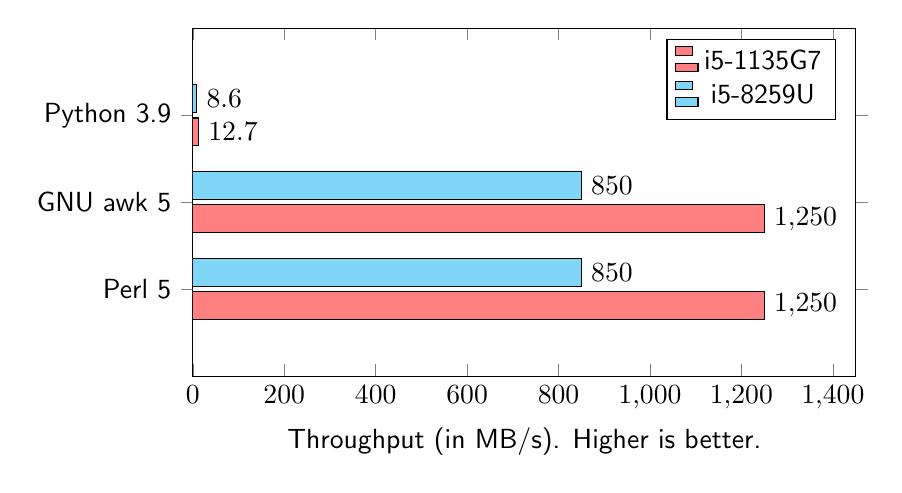
\begin{tikzpicture}
		\begin{axis}
			[ 
			xbar, 
			xmin=0, 
			width=10cm,
			height=6cm, 
			enlarge y limits=0.5, 
			xlabel={Throughput (in MB/s). Higher is better.},
			xmax=1450,
			%ylabel={Language},
			symbolic y coords={perl,gawk,python}, 
			yticklabels={Python 3.9,GNU awk 5,Perl 5},
			ytick=data,
			nodes near coords,
			nodes near coords align={horizontal}, 
			legend pos=north east
			]	
			\addplot[fill=red!50] coordinates {(12.7,python) (1250,gawk) (1250,perl)}; 
			\addplot[fill=cyan!50] coordinates {(8.6,python) (850,gawk) (850,perl)};
			\legend{i5-1135G7,i5-8259U};
		\end{axis} 
	\end{tikzpicture}
	\label{figure:throughput-comparison}
	
\end{figure}


\bigskip

To draw plots, you will need the \quotePkg{pgfplots} package:
\lstinputlisting[language=tex]{include/featured/pkg-pgfplots.tex}


We will not teach you how to draw plots, because the subject is extremely vast. \\



\section{Add an image}

We can add images to our \LaTeX\ files thanks to the \quoteCmd{includegraphics} command from the \quotePkg{graphics} package:
\lstinputlisting[language=tex]{include/featured/pkg-graphics.tex}


Example:
\begin{lstlisting}[language=tex]
\includegraphics{path/to/image-file}
\end{lstlisting}


\begin{figure}[h]
	\caption{Example: adding an image to a document}
	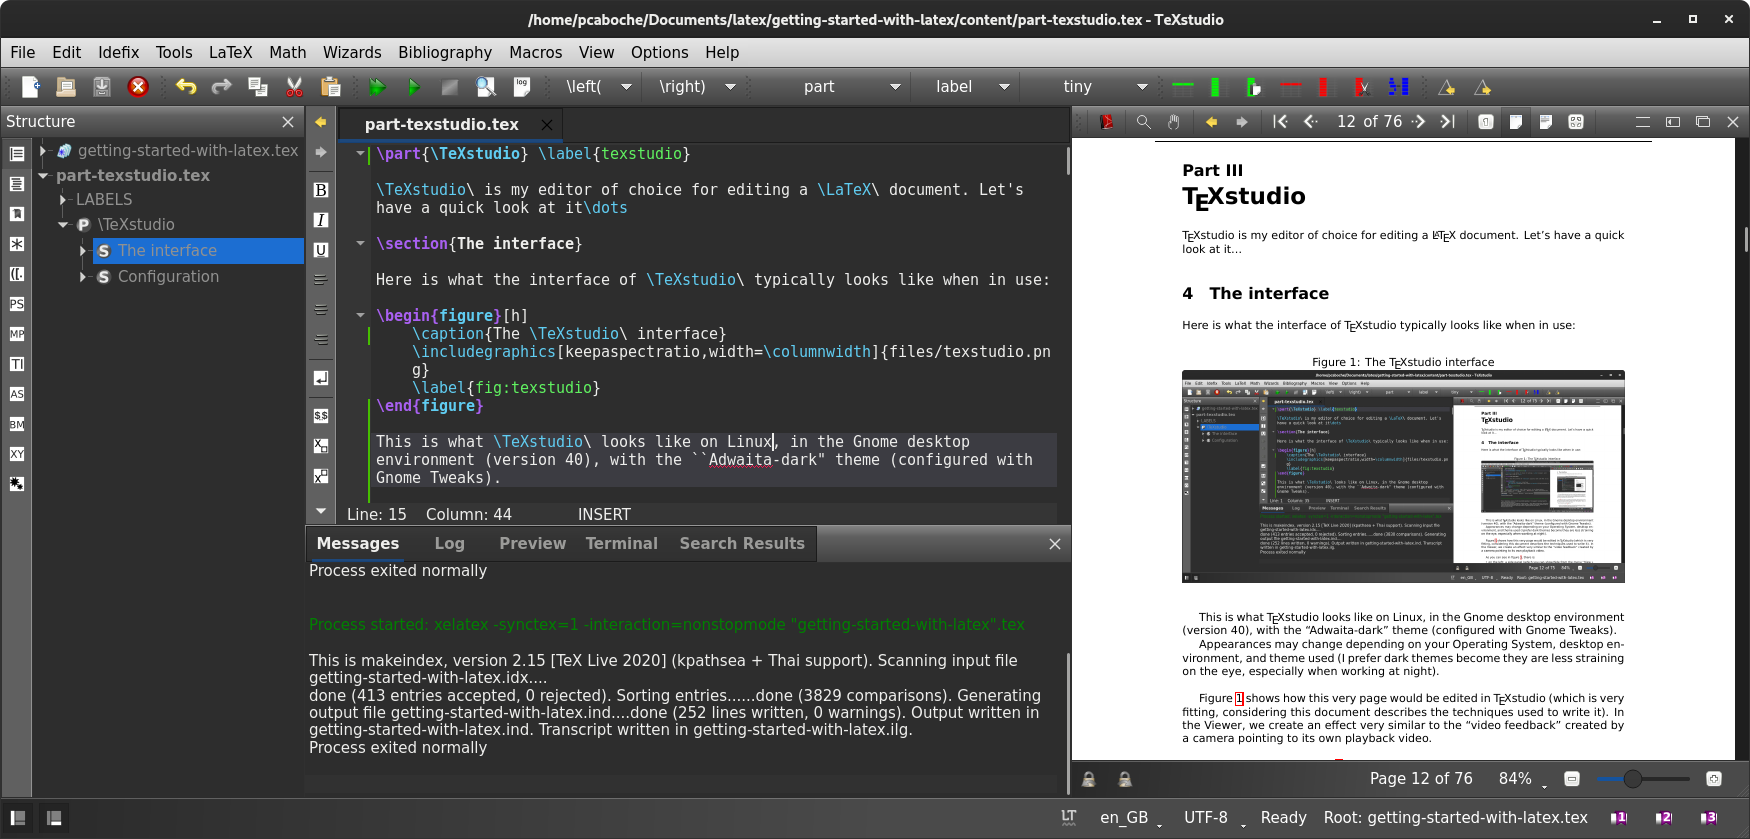
\includegraphics[keepaspectratio,width=\columnwidth]{files/texstudio.png}
\end{figure}


\bigskip

To learn more about \quoteCmd{includegraphics}: \\
\url{https://latexref.xyz/_005cincludegraphics.html}



\subsection{Resize an image to fit the page}

To resize an image to fit the page width, in \quoteCmd{includegraphics} we set the parameters \texttt{keepaspectratio} and \texttt{width}: \\

\begin{tabular}{p{3cm} p{9cm}}
	\texttt{keepaspectratio} & Will make the graphic as large as possible, without distortion, within the constraints of \texttt{width}, \texttt{height}. \texttt{totalheight}. \newline \\
	\texttt{width} & We set the \texttt{width} to either \quoteCmd{linewidth} or \quoteCmd{columnwidth}, and let \texttt{keepaspectratio} resize the image for us. \newline
	\newline
	\quoteCmd{linewidth}: the width of the current line, decreased for each nested list (but because we are not in a list, then it is equal to \quoteCmd{textwidth}, the horizontal width of the page body). \newline
	\newline
	\quoteCmd{columnwidth}: in a two-column document, the width of a column (in a two-column document, it is equal to \quoteCmd{textwidth}). \\
\end{tabular}

\bigskip

Example:
\begin{lstlisting}[language=tex]
\includegraphics[keepaspectratio,width=\columnwidth]{path/to/image-file}
\end{lstlisting}


\newpage


\section{Figures} \label{figures}

Figures are used for easy reference of plots, images, and other visual elements. Figures can be listed in a list of figures, usually at the end of a document. \\

We will study the code associated with figure \ref{figure:throughput-comparison}. \\


Here is the code in question:
\lstinputlisting[language=tex]{include/featured/example-plot-awk-speed.tex}



The content of a figure is contained in a \quoteEnv{figure} environment. The \texttt{[h]} indicates that we want to anchor the figure ``here" (at the location where it has been declared in the document). \\

Then we define the \quoteCmd{caption} of the figure (which will also appear in the list of figures, if one is defined in the document).

Then the command \quoteCmd{centering} indicates that the figure is to be centered in the page. \\

Then we insert the plot itself (which I am not going to describe, that would take too long).

Finally, after the plot, we insert a label. Notice that the ID for the figure starts with ``\texttt{figure:}". This is a convention which allows to easily identify the figures.


\section{List of figures}

We can easily add a list of figures (preferably at the end of the document) with the \quoteCmd{listoffigures} command:
\begin{lstlisting}[language=tex]
\listoffigures
\end{lstlisting}




\newpage
%%%%
%% Copyright 2022 Pierre S. Caboche
%% All rights reserved
%%%%

\part{Extras}

In this part, we list some techniques, as well as some very useful packages (which I actually used in this document) that didn't get to have their own chapter\dots


\section{Other useful packages}

\subsection{Adding web links with \texttt{hyperref}}

The \quotePkg{hyperref} package defines the \quoteCmd{url} command, which allows to add links to web pages. \\

Here is how to import the package:
\lstinputlisting[language=tex]{include/featured/pkg-hyperref.tex}

\bigskip

The \quoteCmd{url} command is very straightforward:
\lstinputlisting[language=tex]{include/featured/example-url.tex}

Result: \\
\url{www.example.com}



\bigskip


\subsection{Ordinal numbers with \texttt{nth}}

The \quotePkg{nth} package is very useful to print ordinal numbers in English (\nth{1}, \nth{2}, \nth{3}, \nth{4}\dots)\\

Here is how to import the package, with the ordinal mark set to be \emph{superscripted}:
\lstinputlisting[language=tex]{include/featured/pkg-nth.tex}

Here are some examples:
\lstinputlisting[language=tex]{include/featured/example-nth.tex}

And here is the result: \\
\nth{1}, \nth{2}, \nth{3}, \nth{4}, \nth{21}, \nth{22}, \nth{23}, 
\nth{101}, \nth{1001}, \nth{1002}, \nth{1000001}
\\


Without \quoteCmd{nth}, you would have to use the \quoteCmd{textsuperscript} command. \\



\newpage

With languages other than English, you would have to use the \quoteCmd{textsuperscript} command (when applicable). For example in French: \\
1\textsuperscript{er} -- premier (masculine), 
1\textsuperscript{ère} -- première (feminine),
2\textsuperscript{ème} -- deuxième, 
3\textsuperscript{ème} -- troisième\dots

\lstinputlisting[language=tex]{include/featured/example-nth-french.tex}

As you can see, this is more complicated in French. \\

Not only do you have to cater for masculine/feminine/plural, but there are other rules. For example, ``\nth{2}" normally translates to << deuxième >> if there are more than two elements, but translates to << second(e) >> if there are more than two elements. \\

This goes to show that the \quotePkg{nth} package may not have an equivalent in other languages.



\newpage
%%%%
%% Copyright 2022 Pierre S. Caboche
%% All rights reserved
%%%%


\section{Conclusion}

This article summarises what I have learned about \LaTeX\ over the past few months, while working on some articles. \\

It all started with a few notes, some tips and tricks about \LaTeX\ that I wanted to remember, and then grew into something much bigger: a guide for people who have never used \LaTeX\ before to be able to write documents or work on their thesis. \\

Interestingly, the writing of this document closely followed the steps described in it\dots\ It starts with opening a template (either a relatively blank template provided by a \TeX\ editor like \TeXstudio, or a standard template that is adopted by the members of the same school, university, organisation\dots) and saving this template in a dedicated folder, where you will store all the files needed for generating the document. \\

Then you start writing down the subjects you want to talk about, and organising them in parts, sections, sub-sections\dots\ So you add a Table-of-Contents to have an overview of the overall structure of your documents. \\

Now that you have some basic plan in place, you start filling out the different parts with ideas. Sometimes the idea is clear enough and a new sentence appears in your document, other times the idea is a bit fuzzy, so you write it down in the form of a comment. \\

Comments are an extremely valuable tool in \LaTeX. They really help in the writing process! \\

\emph{Need to write down an idea that you might want to develop later?} Write down as a comment! \emph{Found an interesting article that you need to explore later?} Write down the reference as a comment! \emph{Not completely satisfied with the phrasing of a certain paragraph?} Comment it out, keep several versions in comments, compare those versions, and eventually you will find the right way to express your idea. \emph{Need to write a note to the people you're collaborating with on the document?} Write a comment!

Comments are fantastic in \LaTeX, and you can put them anywhere. Other text editors only allow you to add comments in a small box in the margin; this is very limiting. It doesn't come close to the power of \LaTeX\ comments and Ctrl+T! (toggle comments on or off, on the selected lines in \TeXstudio) \\

Now that ideas start flowing, and the document starts growing, you organise the content in multiple files of manageable size, which you store in separate folders depending on the file's purpose. \\

And now you start to spot recurring terms, or words that need to appear in the same, consistent format. So you start writing custom \emph{macros} for that, and you also consider adding an index to your document.

Then it's not only recurring terms, but every repeating patterns that you turn into macros, which you can call at will. And it makes your life easier. \\

\newpage

Now that you have a satisfying amount of content, well organised, with lots of cross-references, you want to experiment with the style of the document (unless someone provided you with a template that you need to follow, in that case your document already meets a certain standard of beauty). So you start modifying things like fonts, margin sizes, and probably add a header and footer to the document. 

In any case, it is better to focus on the content of the document first, and modify the style much later. If you want to change the style too early, and in the absence of content, you will have to use some placeholder text (e.g. \LoremIpsum), images, etc. which do not reflect the true content of your document.

So you modify your template much later, when you have at least a dozen pages ready.
\\

And this is how this document came to be! \\

I told you in the abstract that this document was describing how it was written. Although I was initially talking about the different techniques used to generate a document in \LaTeX, in return this also applies to the writing process itself. \\

In any case, I hope you found this article useful, that it helped you on your journey with \LaTeX, or maybe convinced you to try out \LaTeX.



\newpage



\bibliographystyle{apalike}
\bibliography{content/biblio-latex}



\listoftables
\listoffigures



\printindex \label{our-index}

\mbox{} \label{LastPage}

\end{document}
